\documentclass[11pt]{book}
%\usepackage{natbib}
\usepackage[
	backend=bibtex,
	style=numeric,
]{biblatex}
\addbibresource{bibliographie}


\usepackage[english]{babel}
% \usepackage[utf8]{inputenc}
% \usepackage[T1]{fontenc}
\usepackage{fontspec}
\setmainfont{Carlito}
\usepackage[a4paper,left=3cm,right=2.5cm,top=3cm,bottom=3cm, twoside]{geometry}
\usepackage{xcolor}
\usepackage{stmaryrd}
\usepackage{amssymb}
\usepackage{amsmath}
% \usepackage{libertine}
\usepackage{graphicx}
\usepackage{caption}
\usepackage{subcaption}
\usepackage{float}
\usepackage{multirow}
\usepackage{apalike}
\usepackage{minitoc}
\usepackage{tikz}
\usepackage{enumitem}
\usepackage{epigraph}
\usetikzlibrary{shadows.blur}
\usepackage{lscape}
\usepackage{titletoc}
\usepackage{lipsum}
% \usepackage{cite}
\usepackage{booktabs}
\usepackage{arydshln}
\usepackage[nonumberlist]{glossaries}
\usepackage{calc}
\usepackage[]{titlesec} 
\definecolor{linkColor}{HTML}{32a852}
\usepackage[colorlinks=true,citecolor=linkColor,linkcolor=black]{hyperref}
\usepackage{fancyhdr}
\usepackage{lipsum}
\usepackage{listings}
% \usepackage{lmodern} 
% \usepackage{xltabular}
% \usepackage{booktabs}
% \usepackage[normalem]{ulem}
% \useunder{\uline}{\ul}{}
% \usepackage{subfigure}

%%%%%%%%%%%%%%%%%%%%%%%%%%%%%%%%%%%%%%%%%%%%%%%%%%%%%%%%%%%%%%%%%%%%%%%%%%
%%%%%%%%%%%%%%%%%%%%%%%%%%%%%%%%%%%%%%%%%%%%%%%%%%%%%%%%%%%%%%%%%%%%%%%%%%

\lstset{
  % basicstyle=\ttfamily,
  columns=fullflexible,
  frame=single,
  breaklines=true,
  % postbreak=\mbox{\textcolor{red}{$\hookrightarrow$}\space},
}

\definecolor{yourcolor}{HTML}{690843}%{008bb2}

\titleformat{\chapter}[display]
{\normalfont\color{yourcolor}}
{\filleft\huge\color{black}\textsc\chaptertitlename\hspace*{2mm}%
	\begin{tikzpicture}[baseline={([yshift=-.6ex]current bounding box.center)}]
	\node[fill=yourcolor,circle,text=white] {\thechapter};
	\end{tikzpicture}
}
{1ex}
{\titlerule[1.5pt]\vspace*{1.5ex}\Huge\color{black}\textsc}
[]

\titleformat{name=\chapter,numberless}[display]
{\normalfont\color{black}}
{}
{1ex}
{\vspace*{-5cm}\Huge\textsc}
[]

%command to print the acutal minitoc
\newcommand{\printmyminitoc}[1]{%
	\noindent\hspace{1cm}%
	\colorlet{chpnumbercolor}{black}%
	\begin{tikzpicture}
	\node(s){
		\begin{minipage}{.9\linewidth}%minipage trick
		\printcontents[chapters]{}{1}{}
		\end{minipage}
	};
	{
		\color{yourcolor}
		\draw(s.north west)--(s.north east) (s.south west)--(s.south east);
	}
	\end{tikzpicture}
	\vspace*{3ex}
	
	#1
	\vfill
	\pagebreak
}


\newcommand{\HRule}{\rule{\linewidth}{0.7mm}}
\newcommand{\Hrule}{\rule{\linewidth}{0.3mm}}

%%%%%%%%%%%%%%%%%%%%%%%%%%%%%%%%%%%%%%%%%%%%%%%%%%%%%%%%%%%%%%%%%%%%%%%%%%%%%
%%%%%%%%%%%%%%%%%%%%%%%%%%%%%%%%%%%%%%%%%%%%%%%%%%%%%%%%%%%%%%%%%%%%%%%%%%





\begin{document}
	
	\begin{titlepage}
		\begin{center}
			\begin{tabular}{c@{\hskip 1.5cm}c@{\hskip 1.5cm}c@{\hskip 1.5cm}c}
				
\includegraphics[height=1.3cm]{images/Saclay.png} &
				
\includegraphics[height=1.3cm]{images/CFA.jpg} &
                
\includegraphics[height=1.3cm]{images/SFR.png} &
                
\includegraphics[height=1.3cm]{images/Altice.png} \\
			\end{tabular}
		\end{center}
	
		
		\begin{center}

			Université Paris-Saclay\\
			Master 2 Data Science - Apprentissage\\
            2022 - 2023
  
  			\vfill
  			
	 		\HRule \\[0.1cm]
	 		 { \Large {\bfseries Final apprenticeship report} \\
                            and \\
                            {\bfseries Master's thesis} \\
                            Topic extraction from customer call logs using word embeddings and
                            clustering techniques
                            }
	  		\Hrule \\
		
		\end{center}
		
		\vfill
			
		\begin{center}
			\textsc{\Large \textbf{Khang Duy LAI}}\\[1cm] 
		
	
			
			\vspace{1cm}
	
			September 2023
		\end{center}
		
		\vspace{1cm}
			
		
		\begin{center}
			\begin{tabular}{lll}
				 \textsc{\textbf{Romain DADEN}} & Apprenticeship supervisor \\
				 \textsc{\textbf{Kim NGUYEN}} & Academic tutor\\

				
			\end{tabular}\\[1cm]
		\end{center}

	\newpage
	\end{titlepage}



\pagestyle{fancy}

\fancyhead{}

\renewcommand{\chaptermark}[1]{\markboth{\textsc{#1}}{}}


\frontmatter

\tableofcontents
\addcontentsline{toc}{chapter}{Table of contents}

\listoffigures
\addcontentsline{toc}{chapter}{List of figures}

% \listoftables
% \addcontentsline{toc}{chapter}{List of tables}


\mainmatter

\setlength{\parskip}{.7em}

\titlespacing*{\section}{0pt}{.9em}{.8em}
\renewcommand{\baselinestretch}{1.1}


\fancyhead[RO]{\leftmark}
\fancyhead[LE]{\textsc{\chaptername~\thechapter}}

\chapter*{Acknowledgements}
%\startcontents[chapters]
\addcontentsline{toc}{chapter}{Acknowledgements}  

First and foremost, I would like to express my gratefulness and sincere to my supervisor, engineer Romain Daden, for giving me a wonderful opportunity to work and study in this machine learning topic, for the continuous support during my apprenticeship at SFR-Altice and for his patience, motivation and immense knowledge. His guidance helps me to follow the correct path in the time I worked. I could not have imagined having a better supervisor and mentor in my very last and important year of study to finish the Master's program.

My sincere also goes to my extraordinary team at SFR Analytics, who do not hesitate to help me with anything, even helping me with difficulties in life the very first time I am in France. I will be unable to have such a nice and remarkable apprenticeship without them.

I would like to show my thankfulness to my academic tutor, Kim Nguyen, and to all of my teachers who have been alongside me for two years of my master's at both Université Paris Cité and Université Paris Saclay. It is a great pleasure to be your student.

I would like also to give great respect to the company of Altice SFR, which provide me with a place to work, and the equipment that I use during the apprenticeship, my very kind housemates, as well as my classmate, to help me with the very first day I came to Paris.

Last but not least, I also want to give great gratefulness to my family for giving me a lot of mental as well as financial support. This thesis could not be done without them.




\chapter*{Abstract}
\addcontentsline{toc}{chapter}{Abstract}

This document comprises two distinct segments, starting with an apprenticeship report followed by an in-depth explanation of the master's thesis about the last mission in the list below.

In the initial section, an overview is presented of my work as an apprentice within the company. A brief introduction of the organization is provided, followed by a report of the mission that I have undertaken:

\begin{itemize}
    \item Enhancing Fake and Near-Duplicate Fiber Distribution Point Images Detection.

Investigating and refining methods to recognize counterfeit and near-duplicated fiber distribution point images, avoiding paying for forgery work.

    \item Exploring Feasibility of Migrating Infrastructure to Google Cloud

Evaluating the viability of transferring the existing infrastructure to Google Cloud, harnessing cloud capabilities for improved scalability, efficiency, and innovation.

    \item Categorizing Customer Conversations from SFR call center data via NLP Techniques.

Employing Natural Language Processing techniques to categorize and extract insights from customer interactions, thereby enhancing service quality and decision-making.

\end{itemize}

Customer satisfaction is one of the most important factors of any company in the market nowadays. The collection of valued data from the conversations with the customer from the call center and extracting the meaning out of it has been done by almost every enterprise to improve competitive advantage in the market with other competitors. In the second segment, This article dives into more detail about the analysis of transcribed calls document of SFR's client, with the desire to find out the topics of the conversation, thereby helping the company to improve customer satisfaction later on. To do so, I will apply a French language model named CamemBERT, a variety of RoBERTa to extract the sentence meaning in a form of a vector in the vector space, and then apply some clustering techniques to cluster conversations into topics. We will find the most important words by using TF-IDF, or define the topic by a representative document that is closest to the centroids.

\textbf{Keywords}: Computer vision, CLIP, Vertex AI, Google Cloud, CamemBERT, Language model, Topic clustering, TF-IDF


\part{Apprenticeship report}
\chapter{Host company introduction}

\startcontents[chapters]
\printmyminitoc{
	In this chapter, I would like to introduce the company that I am currently working on, Société française du radiotéléphone (SFR). It covers the sector of activity, the history of the company, its values and the most important part is how it is related to the master's that I am currently pursuing at Université Paris-Saclay.
}

\section{Sector of Activity}

Société française du radiotéléphone (SFR), is a French telecommunications company. It is the second oldest mobile network operator in France, after Orange and the second largest telecommunications company in France, also behind Orange.

SFR operates in the telecommunications sector, providing a wide range of communication and connectivity services to both individual consumers and businesses. The company's core activities include:

\begin{itemize}

    \item  Mobile services: offers mobile voice and data services, allowing customers to make calls, send messages, and access the internet on their smartphones and other mobile devices.

    \item Fixed-line services: provides fixed-line telephone services, including landline phone connections for homes and businesses.

    \item Internet services: offers broadband and high-speed internet connections, enabling customers to access the internet at home or work.

    \item Television services: deliver television services, including digital TV channels, on-demand content, and interactive features.

\end{itemize}

\begin{figure}[H]
    \centering
    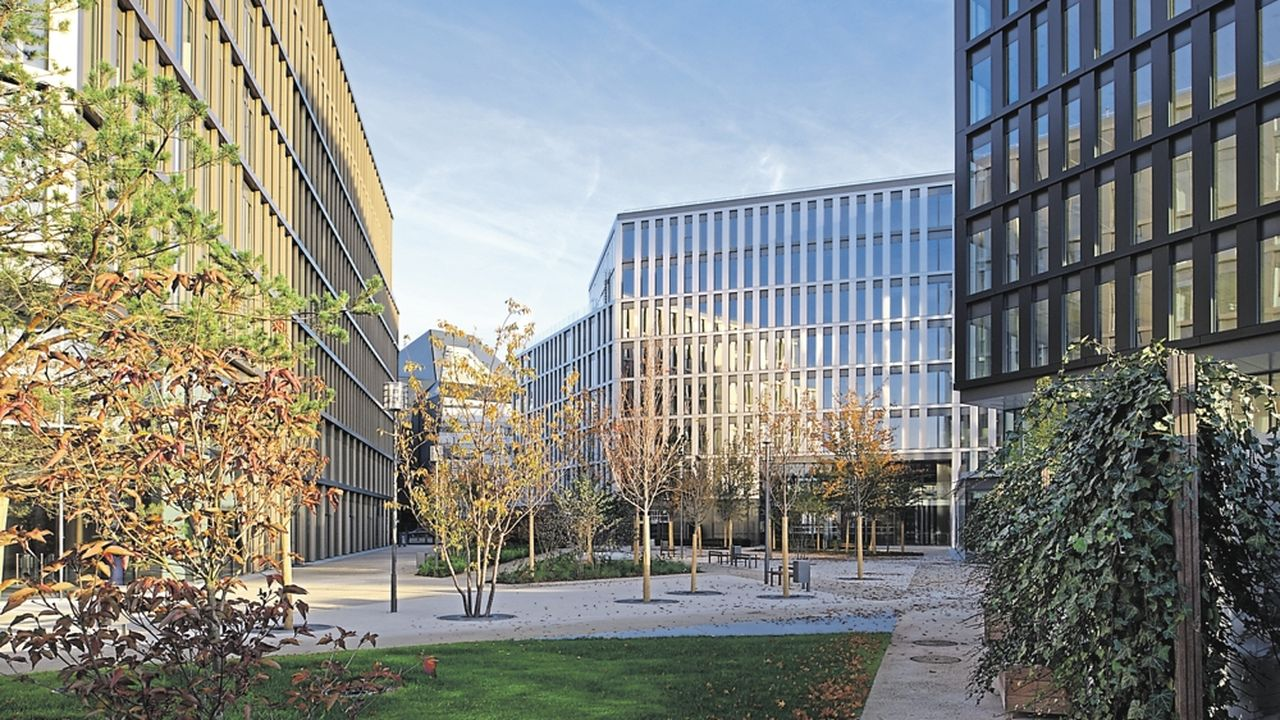
\includegraphics[width=0.9\textwidth]{images/altice-campus.jpg}
    \caption{A part of the current campus at 15ème arrondissement}
    \label{fig:altice_campus}
\end{figure}

SFR is known for its convergence strategy, which involves bundling multiple services, such as mobile, fixed-line, internet, and television, into comprehensive packages for customers seeking integrated communication and entertainment solutions.

Besides the representation of SFR in the Business-to-Consumer market, the company also serves the Business-to-Business market by offering tailored communication and connectivity solutions to support various industries and organizations.

\section{History}

\begin{figure}[H]
    \centering
    
\includegraphics[width=0.4\textwidth]{images/SFR-Logo-History.jpg} % Replace "example-image.jpg" with the actual filename of your image
    \caption{History of SFR logo over time}
    \label{fig:sfr_logo}
\end{figure}

\begin{itemize}

    \item Founding Years and Early Growth (1987-2000):

SFR was established in 1987 as a subsidiary of Compagnie Générale des Eaux (now Veolia Environnement). The company's inception marked a significant step in introducing mobile telecommunications services to France.

    \item Expansion and Technological Advancements (2000s):

In the early 2000s, SFR launched its 3G (third generation) network, marking a milestone in mobile data services. The company's commitment to innovation and network improvement led to expanded coverage and enhanced service quality.

    \item Mergers and Acquisitions - Altice Era (2014):

In 2014, a major turning point occurred when Altice, a prominent cable and telecom company led by entrepreneur Patrick Drahi, acquired a controlling stake in SFR. This acquisition initiated a period of transformation and strategic repositioning for SFR within the Altice Group.

Under Altice's ownership, SFR underwent a series of changes aimed at convergence and diversification. The company focused on providing bundled services that combined mobile, fixed-line, internet, and television offerings, catering to customers' diverse communication and entertainment needs.

    \item Innovation and 5G Era (2020s):

Continuing its legacy of innovation, SFR, under the guidance of Altice, played a pivotal role in the deployment of 5G technology in France. This next-generation wireless technology promised higher speeds and improved connectivity, further solidifying SFR's position as a technological pioneer in the telecommunications landscape.

Throughout its history, SFR's journey has been closely intertwined with its affiliation with Altice, which brought new strategies, innovation, and growth opportunities. The partnership between SFR and Altice continues to shape the telecommunications landscape in France and beyond.

\end{itemize}

\section{Values}

SFR is built upon a foundation of core values that guide its operations and interactions:


\begin{itemize}

    \item \textbf{Innovation}
    
    SFR fosters a culture of continuous innovation, driving the development of cutting-edge solutions to meet the evolving needs of its customers.
    
    \item \textbf{Customer-Centric}
    
    The company is dedicated to delivering exceptional customer experiences, placing customer satisfaction at the heart of its strategies.
    
    \item \textbf{Collaboration}
    
    SFR values collaboration and teamwork, both within its internal teams and in partnership with external stakeholders.
    
    \item \textbf{Ethical Conduct}
    
    Ethical behavior and integrity are paramount in all aspects of SFR's operations, ensuring transparency and trust.
    
\end{itemize}

\section{Application of data in business operations}

Data can help businesses measure whether certain actions, products or services are profitable and where their greatest expenses might be. Identifying expenses is often the key to increasing profits because businesses can reduce those expenses and keep more of the revenue they earn.

SFR Analytics is one of the departments at SFR that takes care of data flow and data process. The department is divided into several groups, each group has its mission in the team.

\begin{itemize}
    \item Data science team
    \item Data analyst team
    \item Data governance team
\end{itemize}

I have been arranged to work in the data science team of SFR Analytics.

The main mission of the department is to manage and process the amount of data acquired by other departments to resolve the problem or to enhance the customer experience with the company. These are some of the missions that SFR Analytics is in charge of.

\begin{itemize}
    \item Reducing Churn Rate
    
SFR harnesses the power of AI and machine learning to analyze customer data and behavior patterns. By applying advanced predictive models, the company can identify potential churn indicators with greater accuracy. This enables SFR to proactively address customer concerns, tailor retention strategies, and offer personalized incentives, ultimately reducing churn rates. AI-driven insights empower SFR to anticipate customer needs, enhance service offerings, and strengthen customer relationships.

    \item Image Processing for Infrastructure Optimization
    
In its commitment to delivering optimal network performance, SFR employs AI-powered image processing techniques. By analyzing images and data collected from network infrastructure, AI algorithms can identify potential issues such as equipment damage or environmental factors that might affect network quality. This proactive approach allows SFR to swiftly address maintenance needs, minimize service disruptions, and ensure seamless connectivity for its customers.

    \item Natural Language Processing (NLP) in Call Centers
    
SFR revolutionizes its call center operations through the integration of natural language processing (NLP). AI-driven NLP models enable the automated analysis of customer interactions, extracting valuable insights from voice conversations, emails, and chat interactions. This not only enhances customer service quality by providing real-time assistance but also enables SFR to gain a deeper understanding of customer sentiments, preferences, and pain points. By leveraging NLP, SFR can fine-tune its services, optimize call center workflows, and continuously improve its offerings based on customer feedback.

    \item Predictive Analytics for Network Management
    
AI-driven predictive analytics play a vital role in optimizing SFR's network management. By analyzing vast amounts of network data, AI algorithms can forecast network congestion, identify potential areas of service degradation, and recommend proactive adjustments to ensure optimal network performance. This data-driven approach enhances user experiences, reduces downtime, and positions SFR as a provider of reliable and high-quality connectivity services.

\end{itemize}

SFR's strategic integration of artificial intelligence and machine learning into its business activities underscores the company's commitment to innovation and customer satisfaction. By leveraging AI-driven insights, SFR enhances its ability to reduce churn, optimize network infrastructure, elevate call center operations, and ensure seamless connectivity. These advancements not only propel SFR's growth but also contribute to its mission of delivering exceptional communication and digital services to its diverse customer base.
\chapter{Missions}

\startcontents[chapters]
\printmyminitoc{
This chapter will specify my roles and responsibilities in the position as a data scientist apprentice at SFR. Additionally, it will introduce the problems that I need to solve and the objective of each mission that I need to achieve at the end of the apprenticeship duration. The details of techniques, the methods that I used, and also the results will be discussed in the next chapter, \autoref{chap:problemsolving}. The current chapter centers on the introduction of the problems and the desired outcomes only.
}

The data science team at SFR Analytics contributes to a wide array of crucial tasks aimed at using the power of data for informed decision-making and strategic insights. The diverse responsibilities of our team contain, but are not limited to, the following:

\begin{itemize}
    \item Data Collection

    Gather, process, and clean large datasets from various sources, including customer interactions, network performance metrics, and user behavior data.
    
    \item Data Exploration

    Conduct data exploration to identify trends, patterns, and insights that can inform business strategies and improve operations.
    
    \item Predictive Modeling and Machine Learning

    Develop and implement machine learning models to predict customer behavior, optimize network performance, reduce churn rate and drive various business outcomes.
    
    \item Impact Assessment and Strategy

    Measure the impact of data science initiatives on key performance indicators and contribute to the development of business strategies.
\end{itemize}

As part of the Data Science team, each member is assigned specific responsibilities aligned with their expertise and the organization's goals. Together with other teams, we contribute to the company using data-driven techniques to improve efficiency and productivity.

\section{Roles and position}

As a data scientist at the Data Science Team of SFR Analytics, I contribute to the company's data-driven decision-making processes and strategic initiatives. SFR is committed to delivering cutting-edge communication and connectivity services to its diverse customers. In line with this mission, SFR Analytics serves as the analytical arm of the organization, dedicated to extracting valuable insights from the vast volumes of data generated within the telecommunications landscape.

Within this context, my assignment centers on these 3 main problems:

\begin{itemize}
    \item Improve fake and near-duplicate fiber distribution point image detection.
    \item Research the feasibility of moving existing infrastructure to Google Cloud.
    \item Categorize topics from the conversation with customers from the call center using NLP techniques.
\end{itemize}

These problems have been identified as necessary and, once addressed, have the potential to drive a positive impact for both SFR and its customers.

Throughout my period as an apprentice in the company, my duty in the team changed through time, from improving existing models to doing research and reporting on the feasibility of bringing existing infrastructure to the cloud, as well as creating new directions for the group in the future.


\section{In charge projects}

\subsection{Fiber distribution point fake and near-duplicated images detection}

SFR and other operators (Orange, Free and Bouygues) have a network of fiber aggregation points all over France. Because of the size of the network, the expense of maintenance and modernization is huge. In order to reduce the cost, It is more optimized to collaborate and share the network between operators. Orange, Free and Bouygues can use SFR fiber distribution points and vice versa.

\begin{figure}[H]
    \centering
    \begin{subfigure}{0.3\textwidth}
        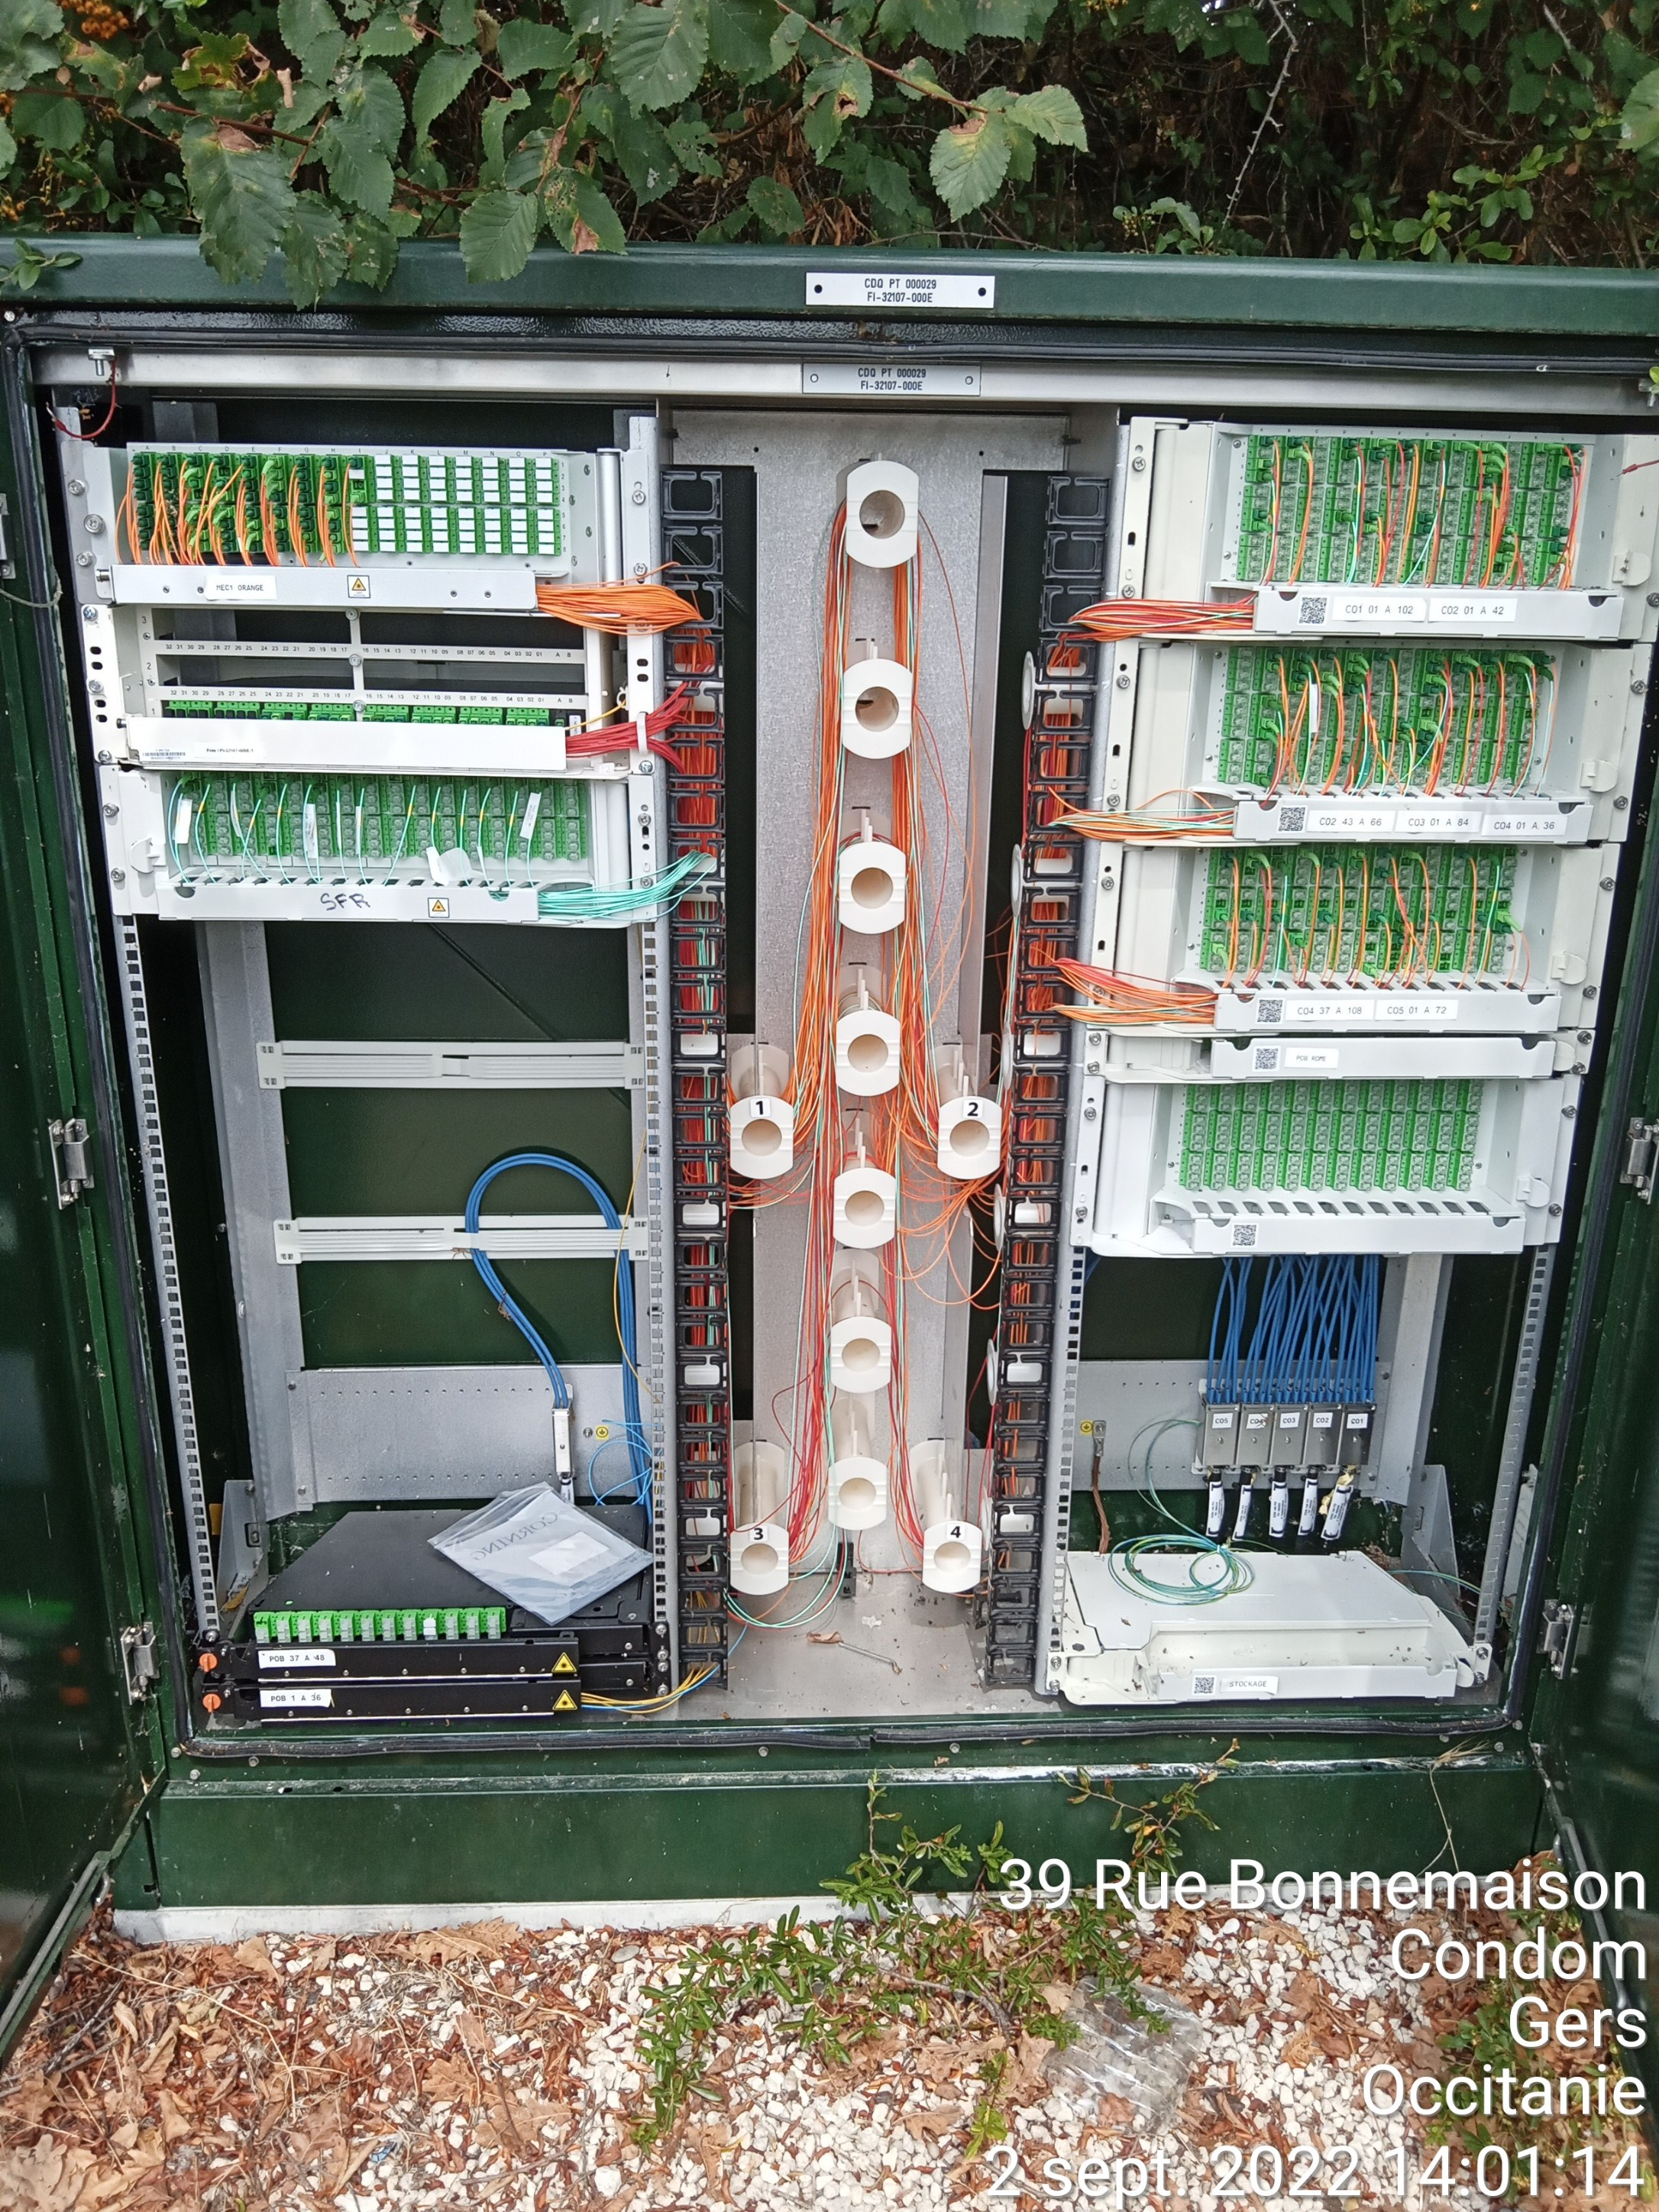
\includegraphics[width=\linewidth]{images/pm_example.jpg}
        \caption{PM no 1}
    \end{subfigure}
    \begin{subfigure}{0.3\textwidth}
        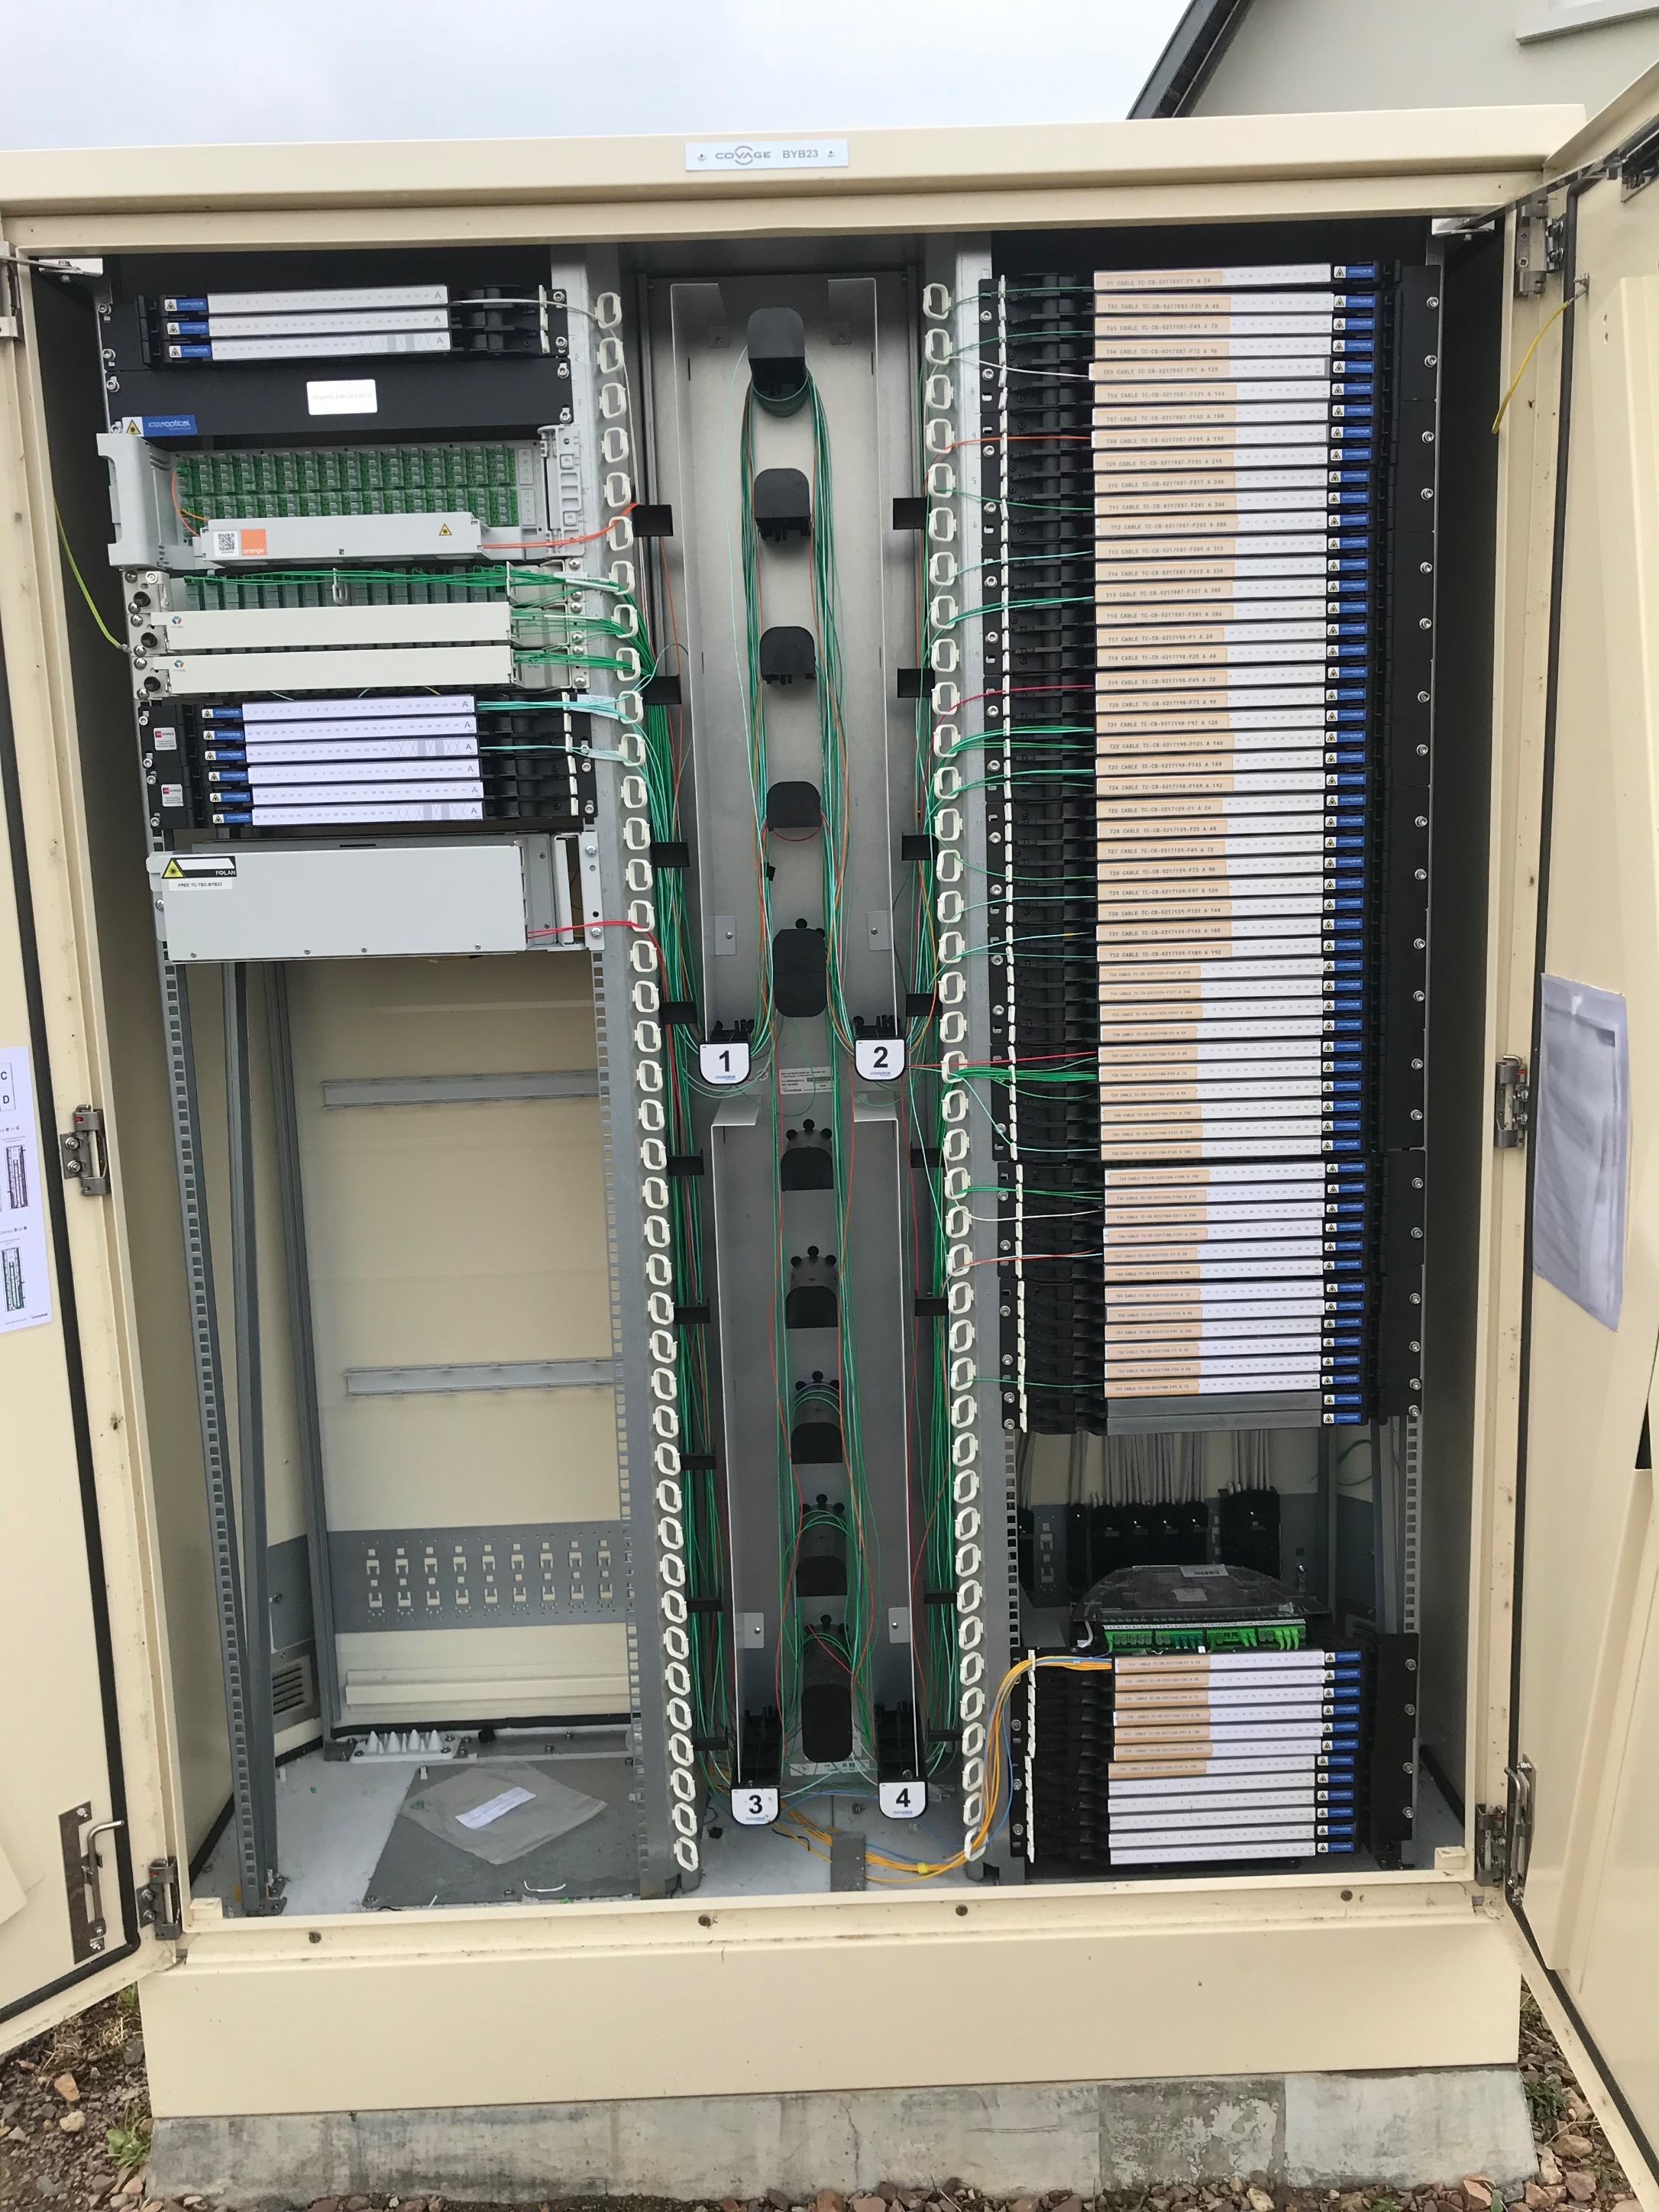
\includegraphics[width=\linewidth]{images/pm_example_2.jpg}
        \caption{PM no 2}
    \end{subfigure}
    \begin{subfigure}{0.3\textwidth}
        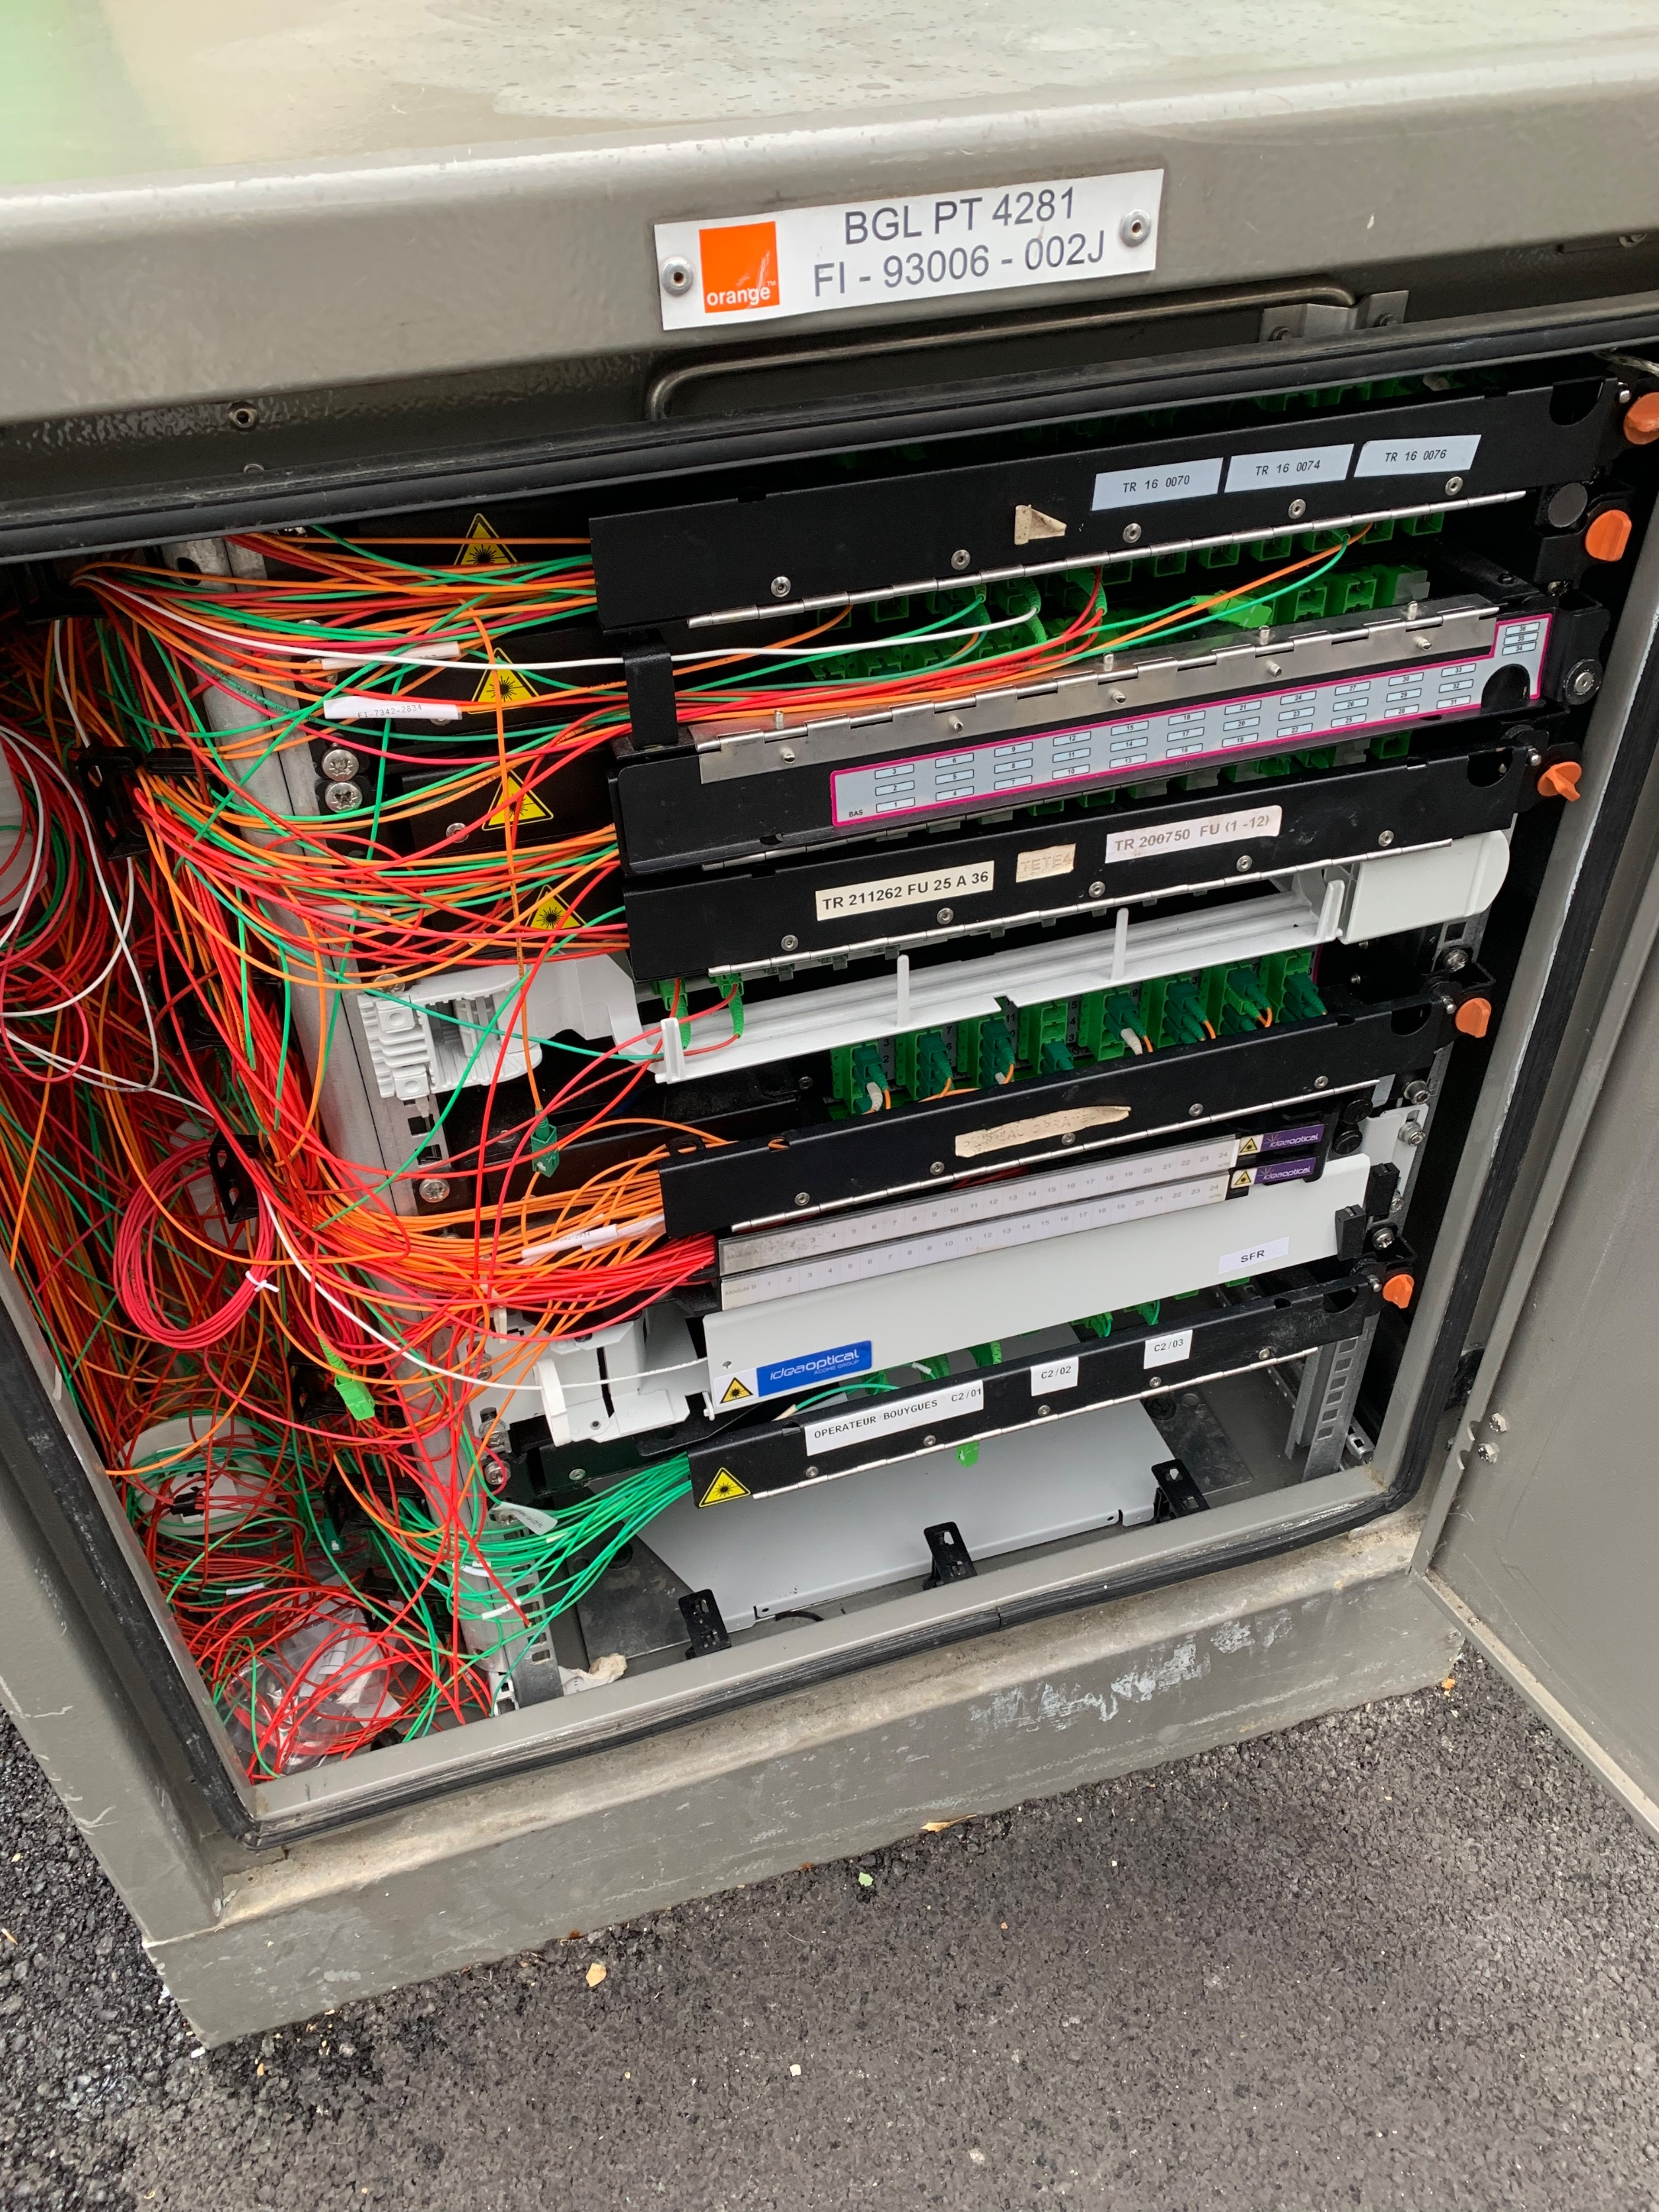
\includegraphics[width=\linewidth]{images/pm_example_3.jpg}
        \caption{PM no 3}
    \end{subfigure}
    \begin{subfigure}{0.5\textwidth}
        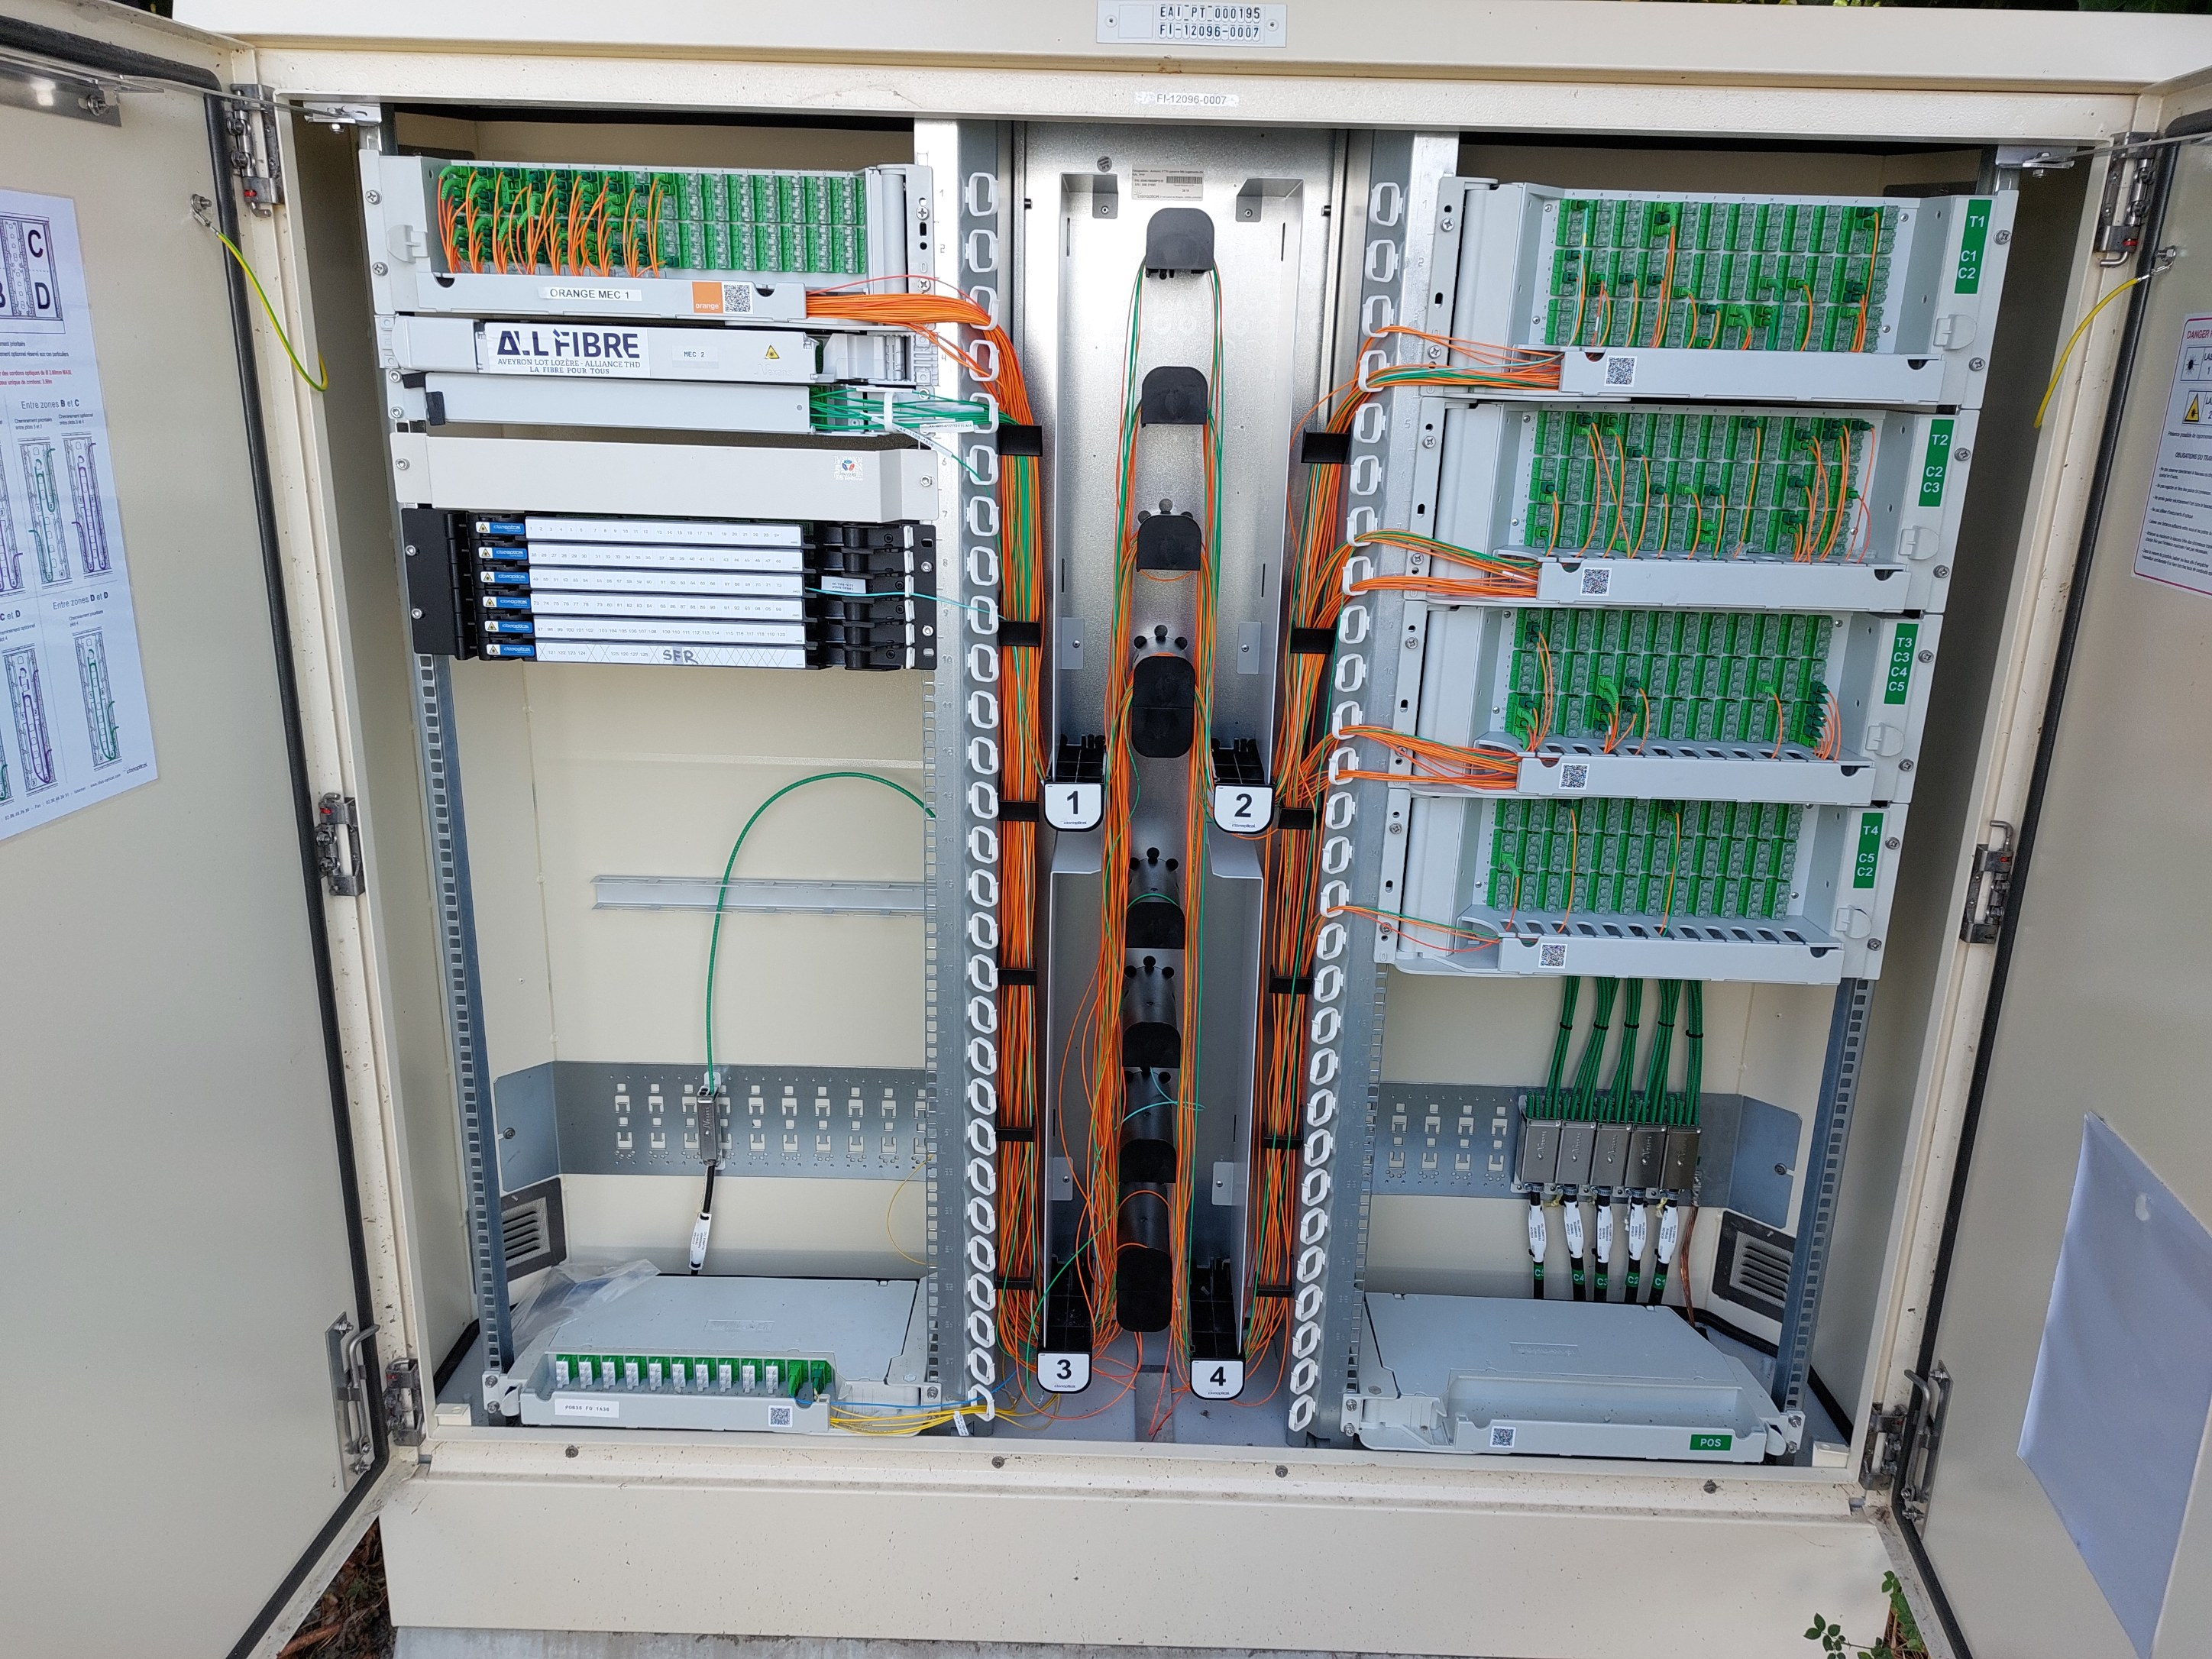
\includegraphics[width=\linewidth]{images/pm_example_4.jpg}
        \caption{PM no 4}
    \end{subfigure}
    \caption{Example of fiber distribution points}
    \label{fig:pm}
\end{figure}

Each point of the network is critical for the region in which it is located. With hundreds of thousands of points, it is difficult to do the maintenance and modernization of the network without collaborating with other companies or outsourcing it to third parties. The work on the fiber distribution point is processed by technicians who are not necessarily staff of SFR, but they could be also staff of such outsourcing companies and the operators will pay the fee for these companies or these independent technicians according to the workload.

To validate their work, an internal application has been used by the technicians to take a picture of their work and according to the image before and after of the fiber distribution point. However, although most of the technicians are honest, some of them do not. They could take a picture once and reupload their previous work several times in order to have validated several times.

It is necessary to build a system that can detect fake and near-duplicate images to prevent technicians from abusing the system. In 80\% of the reupload cases, technicians upload the same image that they have uploaded before. In this case, we could quickly resolve the problem by building a database of image fingerprints and comparing the fingerprints of the new images with it.

In the other 20\%, The images could be changed slightly by the technicians before re-uploading. It includes techniques following:

\begin{itemize}
    \item Slightly rotate the image
    \item Flip the image
    \item Put the image in slide a color box
\end{itemize}

It could be difficult for the system to use the exact image fingerprint because the images have been retouched. If we put the threshold too high, some of the forgery images will pass the system, and if the threshold is set too low, it will trigger false alarms.

The output of this project is to resolve this problem by using computer vision and deep learning techniques.

\subsection{Research the feasibility of moving the team's infrastructure to the Google Cloud}

In response to the evolving demands of a dynamic technological landscape, SFR Analytics is considering a shift from its existing local server infrastructure to a cloud-based model. This move aims to address current challenges and leverage the benefits offered by cloud computing.

The existing local server setup at SFR presents several challenges that impact efficiency, scalability, and operational agility. Moving infrastructure to Google Cloud offers a multitude of benefits that can significantly impact an organization's operations, scalability, and overall efficiency. Here are some key advantages of making this transition:


\begin{itemize}
    \item Scalability and Flexibility: Local servers are limited in their ability to scale on-demand, hindering the organization's ability to handle varying workloads effectively. Cloud services enable seamless scaling of resources, allowing SFR to adapt to changing workloads efficiently.
    
    \item High Costs: The capital expenditure associated with maintaining and upgrading local servers contributes to a significant financial burden. Cloud computing operates on a pay-as-you-go model, reducing upfront costs and minimizing ongoing maintenance expenses.

    \item Maintenance Complexity: Ongoing maintenance, updates, and troubleshooting of local servers require dedicated IT resources and time. Cloud providers handle infrastructure maintenance, updates, and security, freeing up internal IT resources.

    \item Limited Geographic Reach: Local servers may result in latency issues and slower performance for users across different regions. Cloud data centers strategically located worldwide ensure improved latency and enhanced user experiences. Cloud platforms offer built-in redundancy and disaster recovery capabilities, ensuring minimal downtime and data loss.
\end{itemize}

\textbf{Role in Cloud Migration:} Deploying ML and AI Models on Google Cloud Vertex AI

As a contributor to the migration of SFR's infrastructure to Google Cloud, my role revolves around the research of deployment of Machine Learning (ML) and Artificial Intelligence (AI) models on Google Cloud's Vertex AI platform. This initiative aligns with SFR's commitment to leveraging cutting-edge technologies to optimize operations and enhance customer experiences.

\begin{figure}[H]
    \centering
    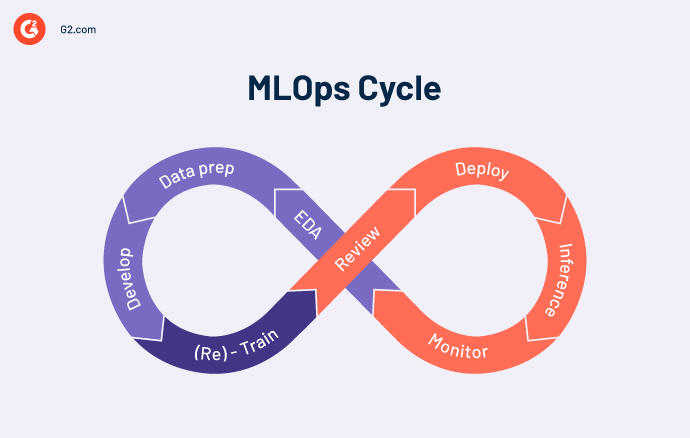
\includegraphics[width=0.7\textwidth]{images/G2CM_FI427_Learn_Article_[Machine_learning_operationalization]_Infographic_image1b_V1.png}
    \caption{MLOps cycle. source: G2.com}
    \label{fig:altice_campus}
\end{figure}

The current workflow of our team is surrounded by the usage of Airflow. The models right now run principally in R script, and we use Airflow to calculate the inferences of the model every day with the supervision of team members. However, some of the work is still manual, and the system stability has been show to be a question. Updating the models also faces differences with a lot of testing before pushing the new models to the production environment

With MLOps, we can solve multiple problems and have various advantages. The most important thing in the deployment of models is the model cycle. Once deployed, it could automatically fetch data needed for training or inference from the database, automatically clean the data and do the preprocessing procedure, automatically evaluate the performance of the new model, and finally automatically deploy the new model to the production environment if critical conditions surpass the set threshold.



\subsection{Apply machine learning techniques on call log from SFR's call center}

As an operator, SFR needs to listen to its customers to find the best and fastest way to improve its services in order to make it more competitive with its competitors. The mission of the customer care center is to listen to the needs of the customer and resolve customer problems that they cannot solve using the dashboard or our chatbot.

It is also essential for the company to understand the problems systematically. One of the ways to do that is to find the topic that is contained in each call from the customer to the call center. Currently, the agents who have the conversation with the customer or the agents who listen to these conversations do the labeling. The data analyst team finds patterns in such conversations and finds insight from such data. 

However, with the current technique of labeling, The conversations could be mislabeled because of the mistake of labelers, or simply because he or she doesn't understand fully the conversation and mislabels it. Therefore, it is necessary to build a system that could automatically detect the common theme of the corpus or suggest the main idea with a list of significant words of conversations.

The objective of the third mission is to use NLP techniques to find the common theme of given transcribed conversations, therefore facilitating the action of labelers with conversations. I will describe this mission in further detail since it is also the topic of the master thesis in the second part of this document.
\chapter{Methods and results}
\label{chap:problemsolving}

\startcontents[chapters]
\printmyminitoc{
}

\section{Fiber distribution point images processing}

\subsection{Example of forgery cases}

Multiple types of forgery images have been discovered. The method of detection should detect the forgery of these cases. The way these images are retouched includes:

\begin{itemize}
    \item Slightly rotate the image
    \item Add into the image a color bar or put it inside a color box.
    \item Cropped
    \item Color shift.
\end{itemize}


\begin{figure}[H]
    \centering
    \begin{subfigure}{0.4\textwidth}
        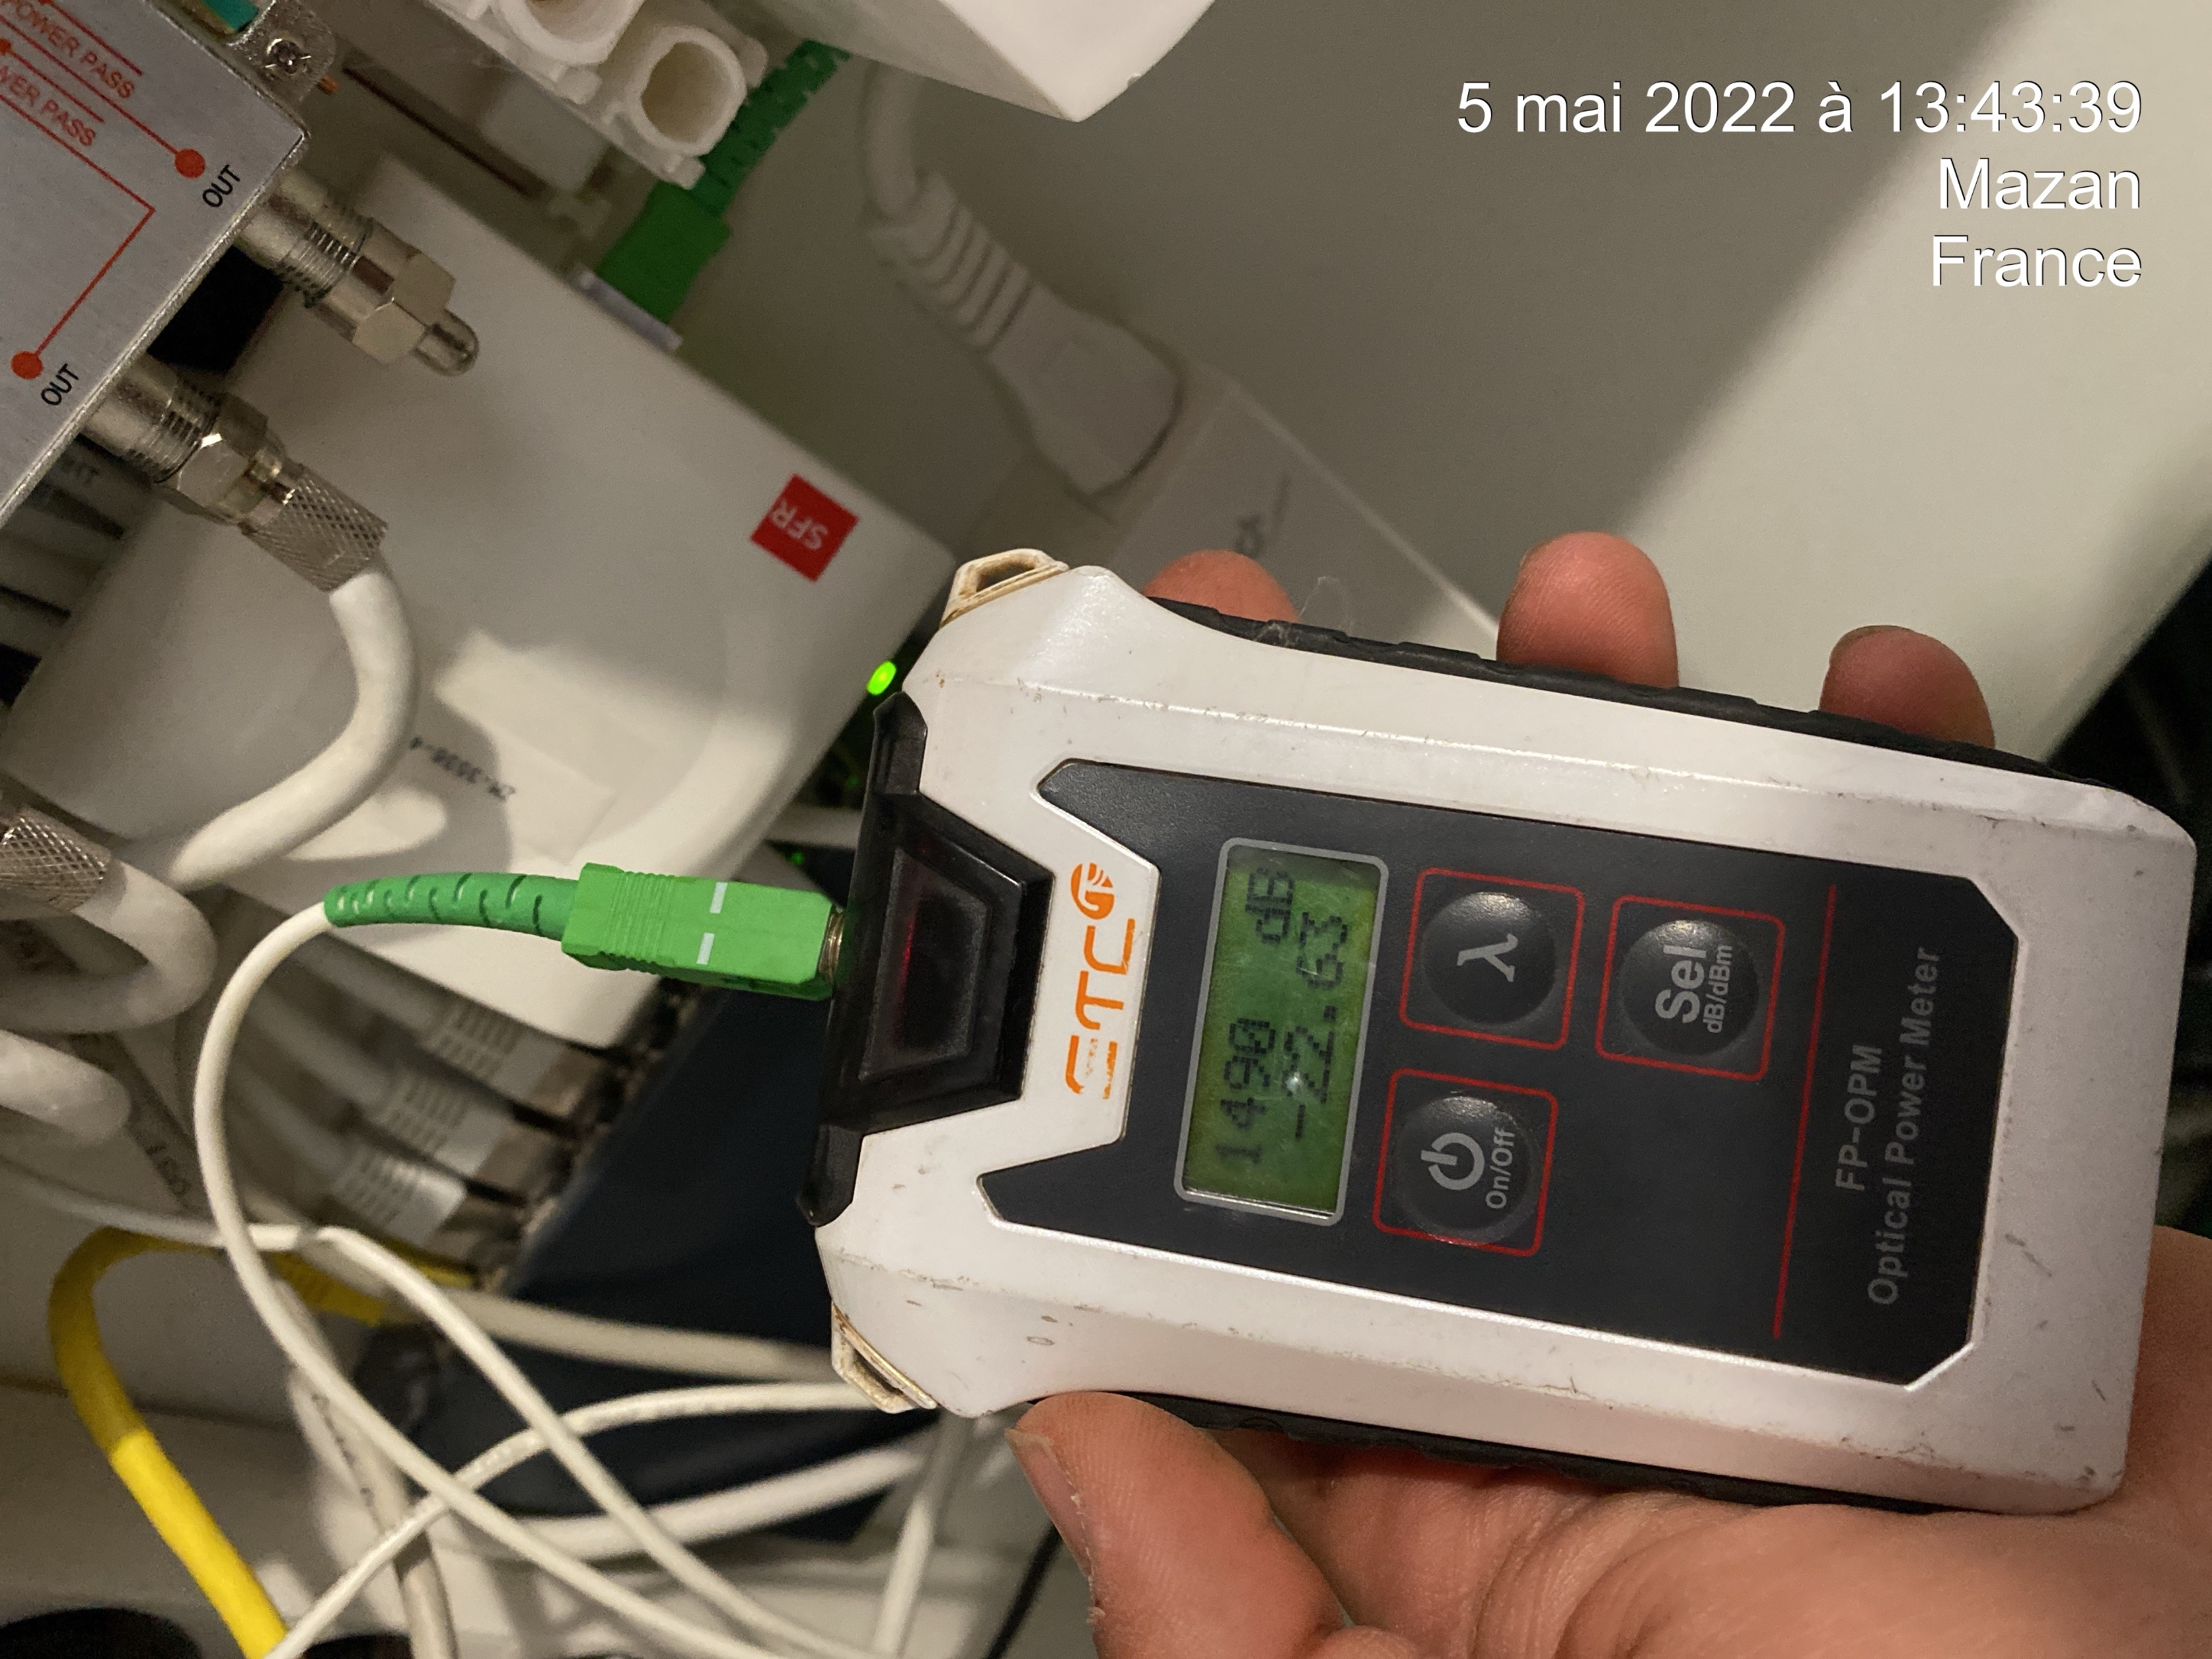
\includegraphics[width=\linewidth]{images/true_positif/t1_true_positif.jpg}
        \caption{Original image}
        \label{fig:true_positif_1}
    \end{subfigure}
    \begin{subfigure}{0.4\textwidth}
        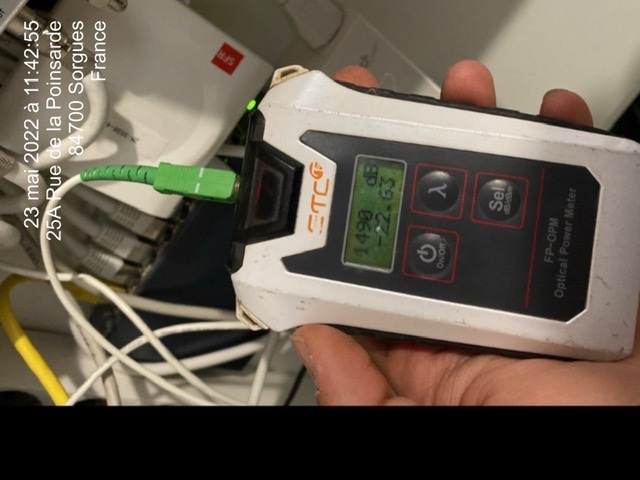
\includegraphics[width=\linewidth]{images/true_positif/t2_true_positif.jpg}
        \caption{Forgery image}
        \label{fig:true_positif_2}
    \end{subfigure}
\end{figure}

As you can see from the example above, the fake image has been cropped a small part at the right side, and then a black bar has been added at the bottom. However, it is also necessary to avoid false alarms. There are a lot of fiber distribution points(PM) that need multiple maintenance. We want to avoid the pictures of the same PM but on different days.

\begin{figure}[H]
    \centering
    \begin{subfigure}{0.3\textwidth}
        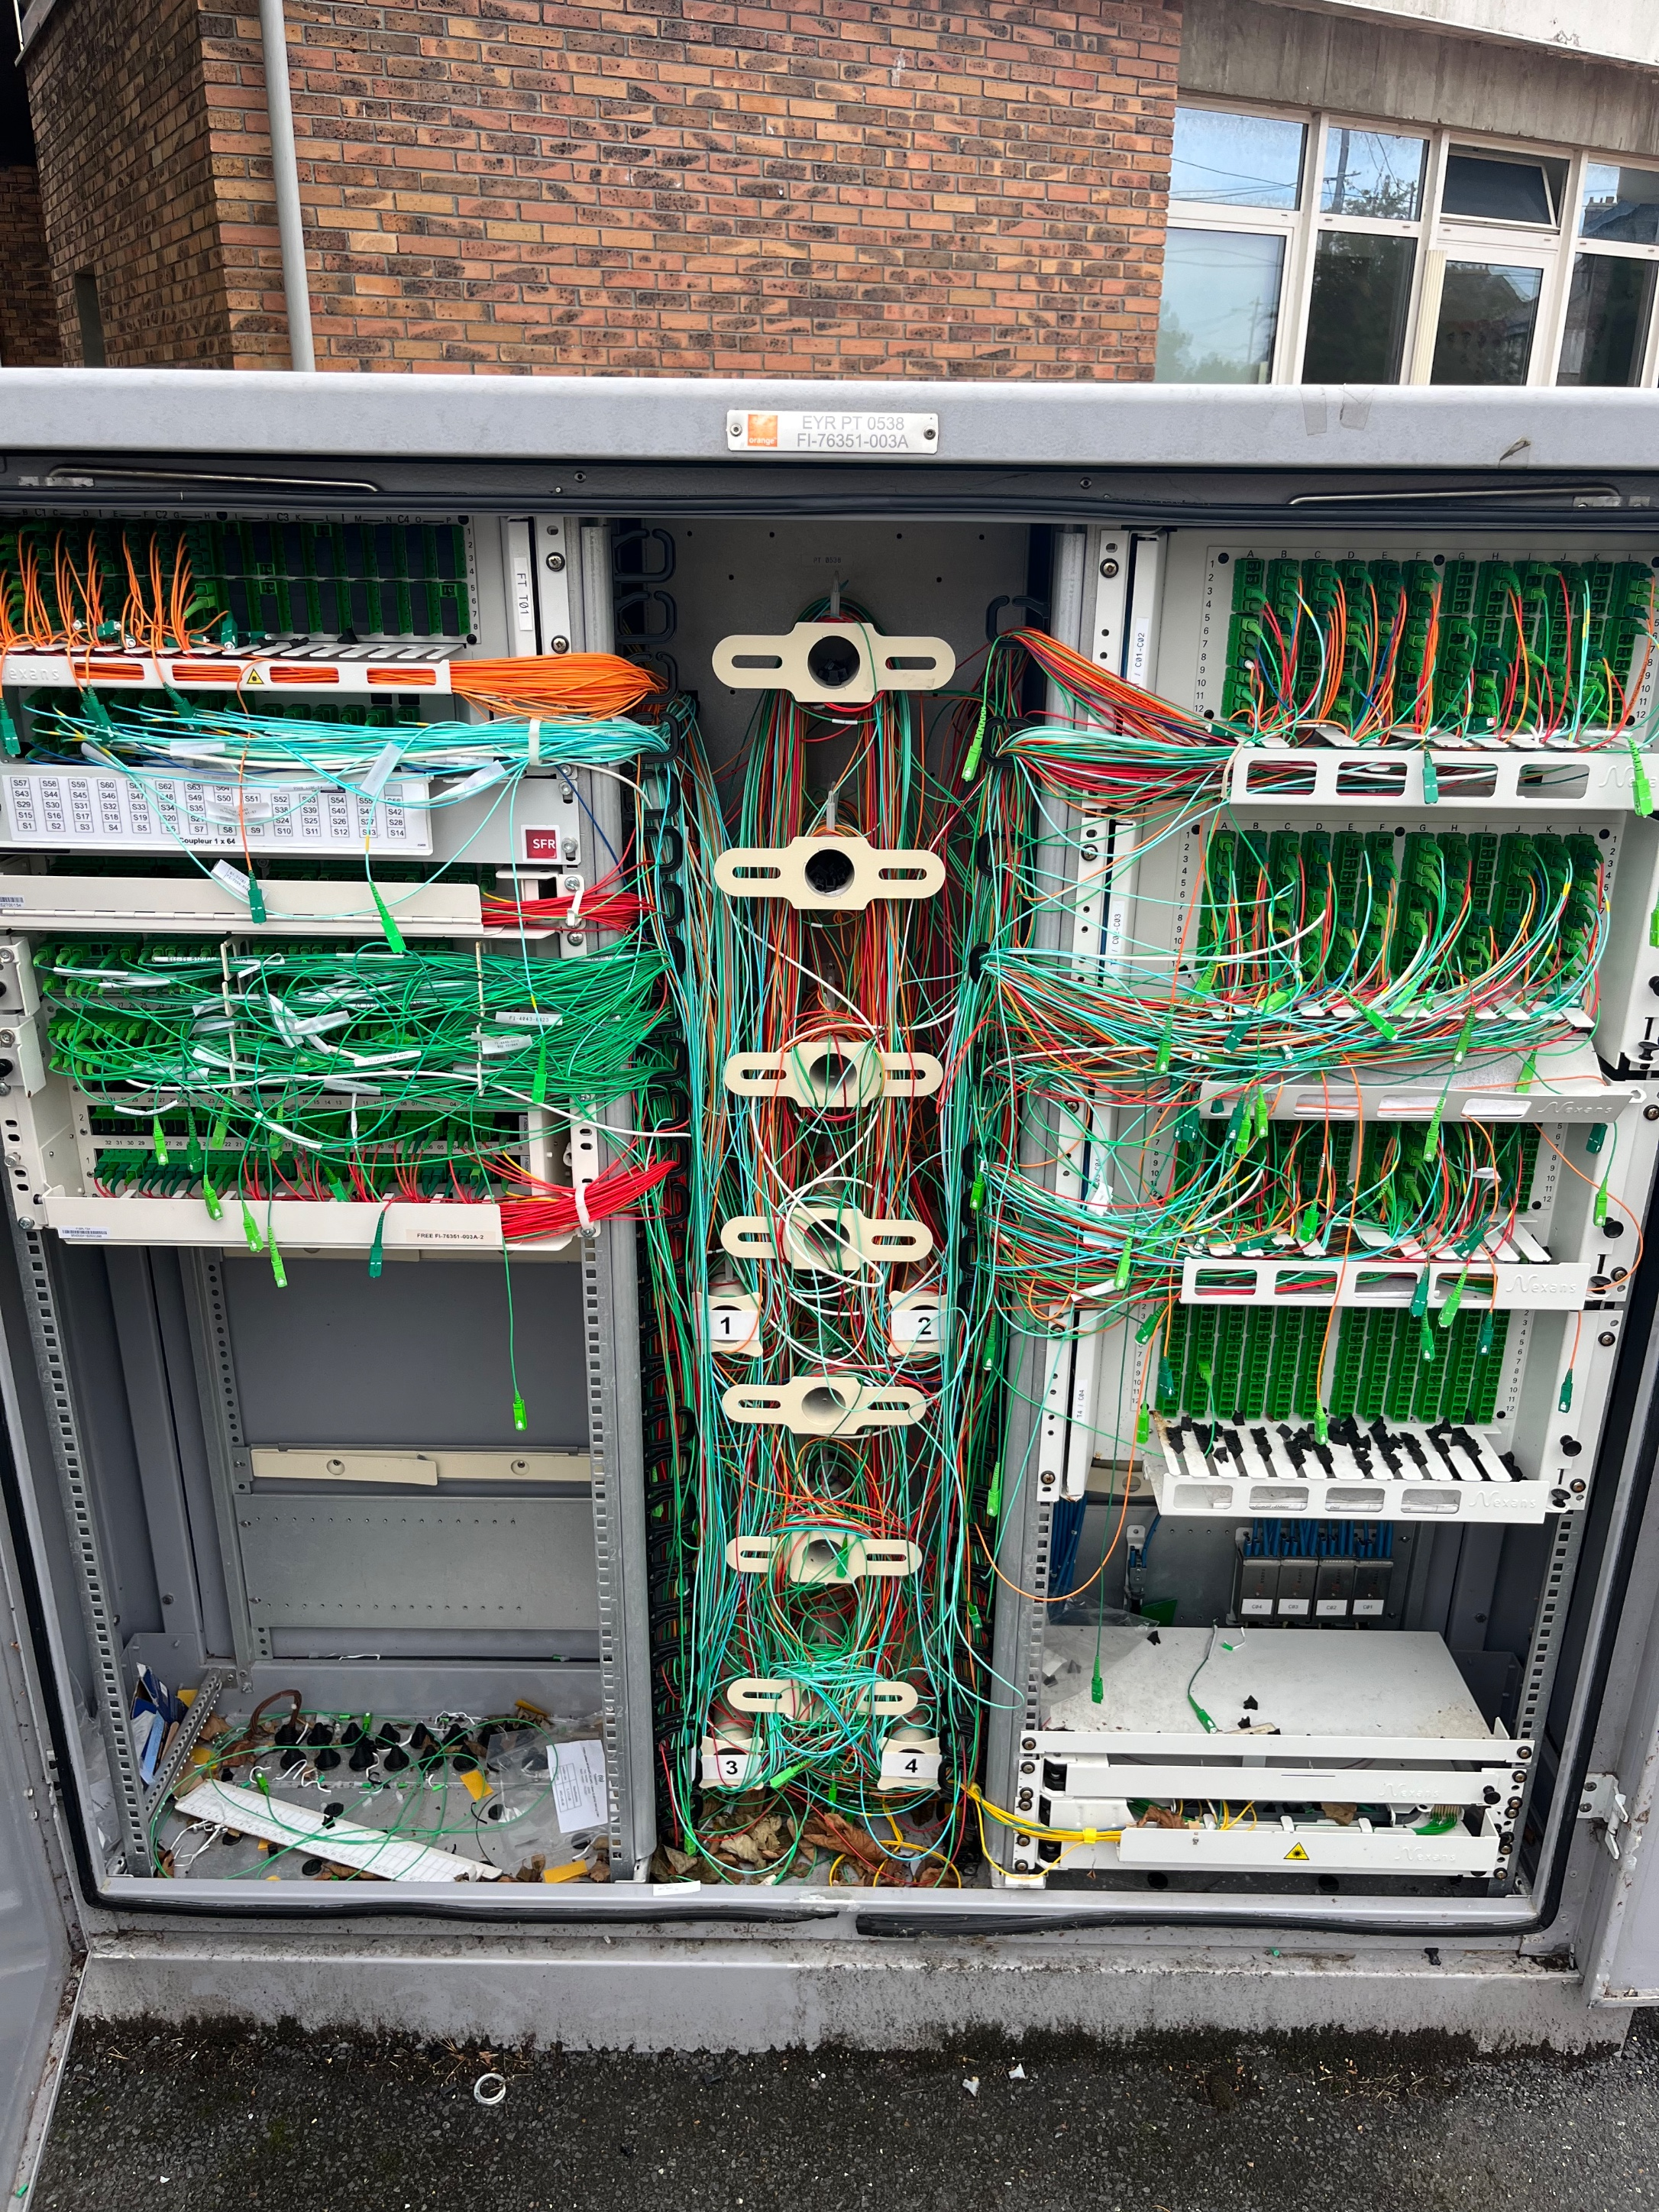
\includegraphics[width=\linewidth]{images/false_positif/5173534_1.jpg}
        \caption{Example of a false alarm - 1}
    \end{subfigure}
    \begin{subfigure}{0.3\textwidth}
        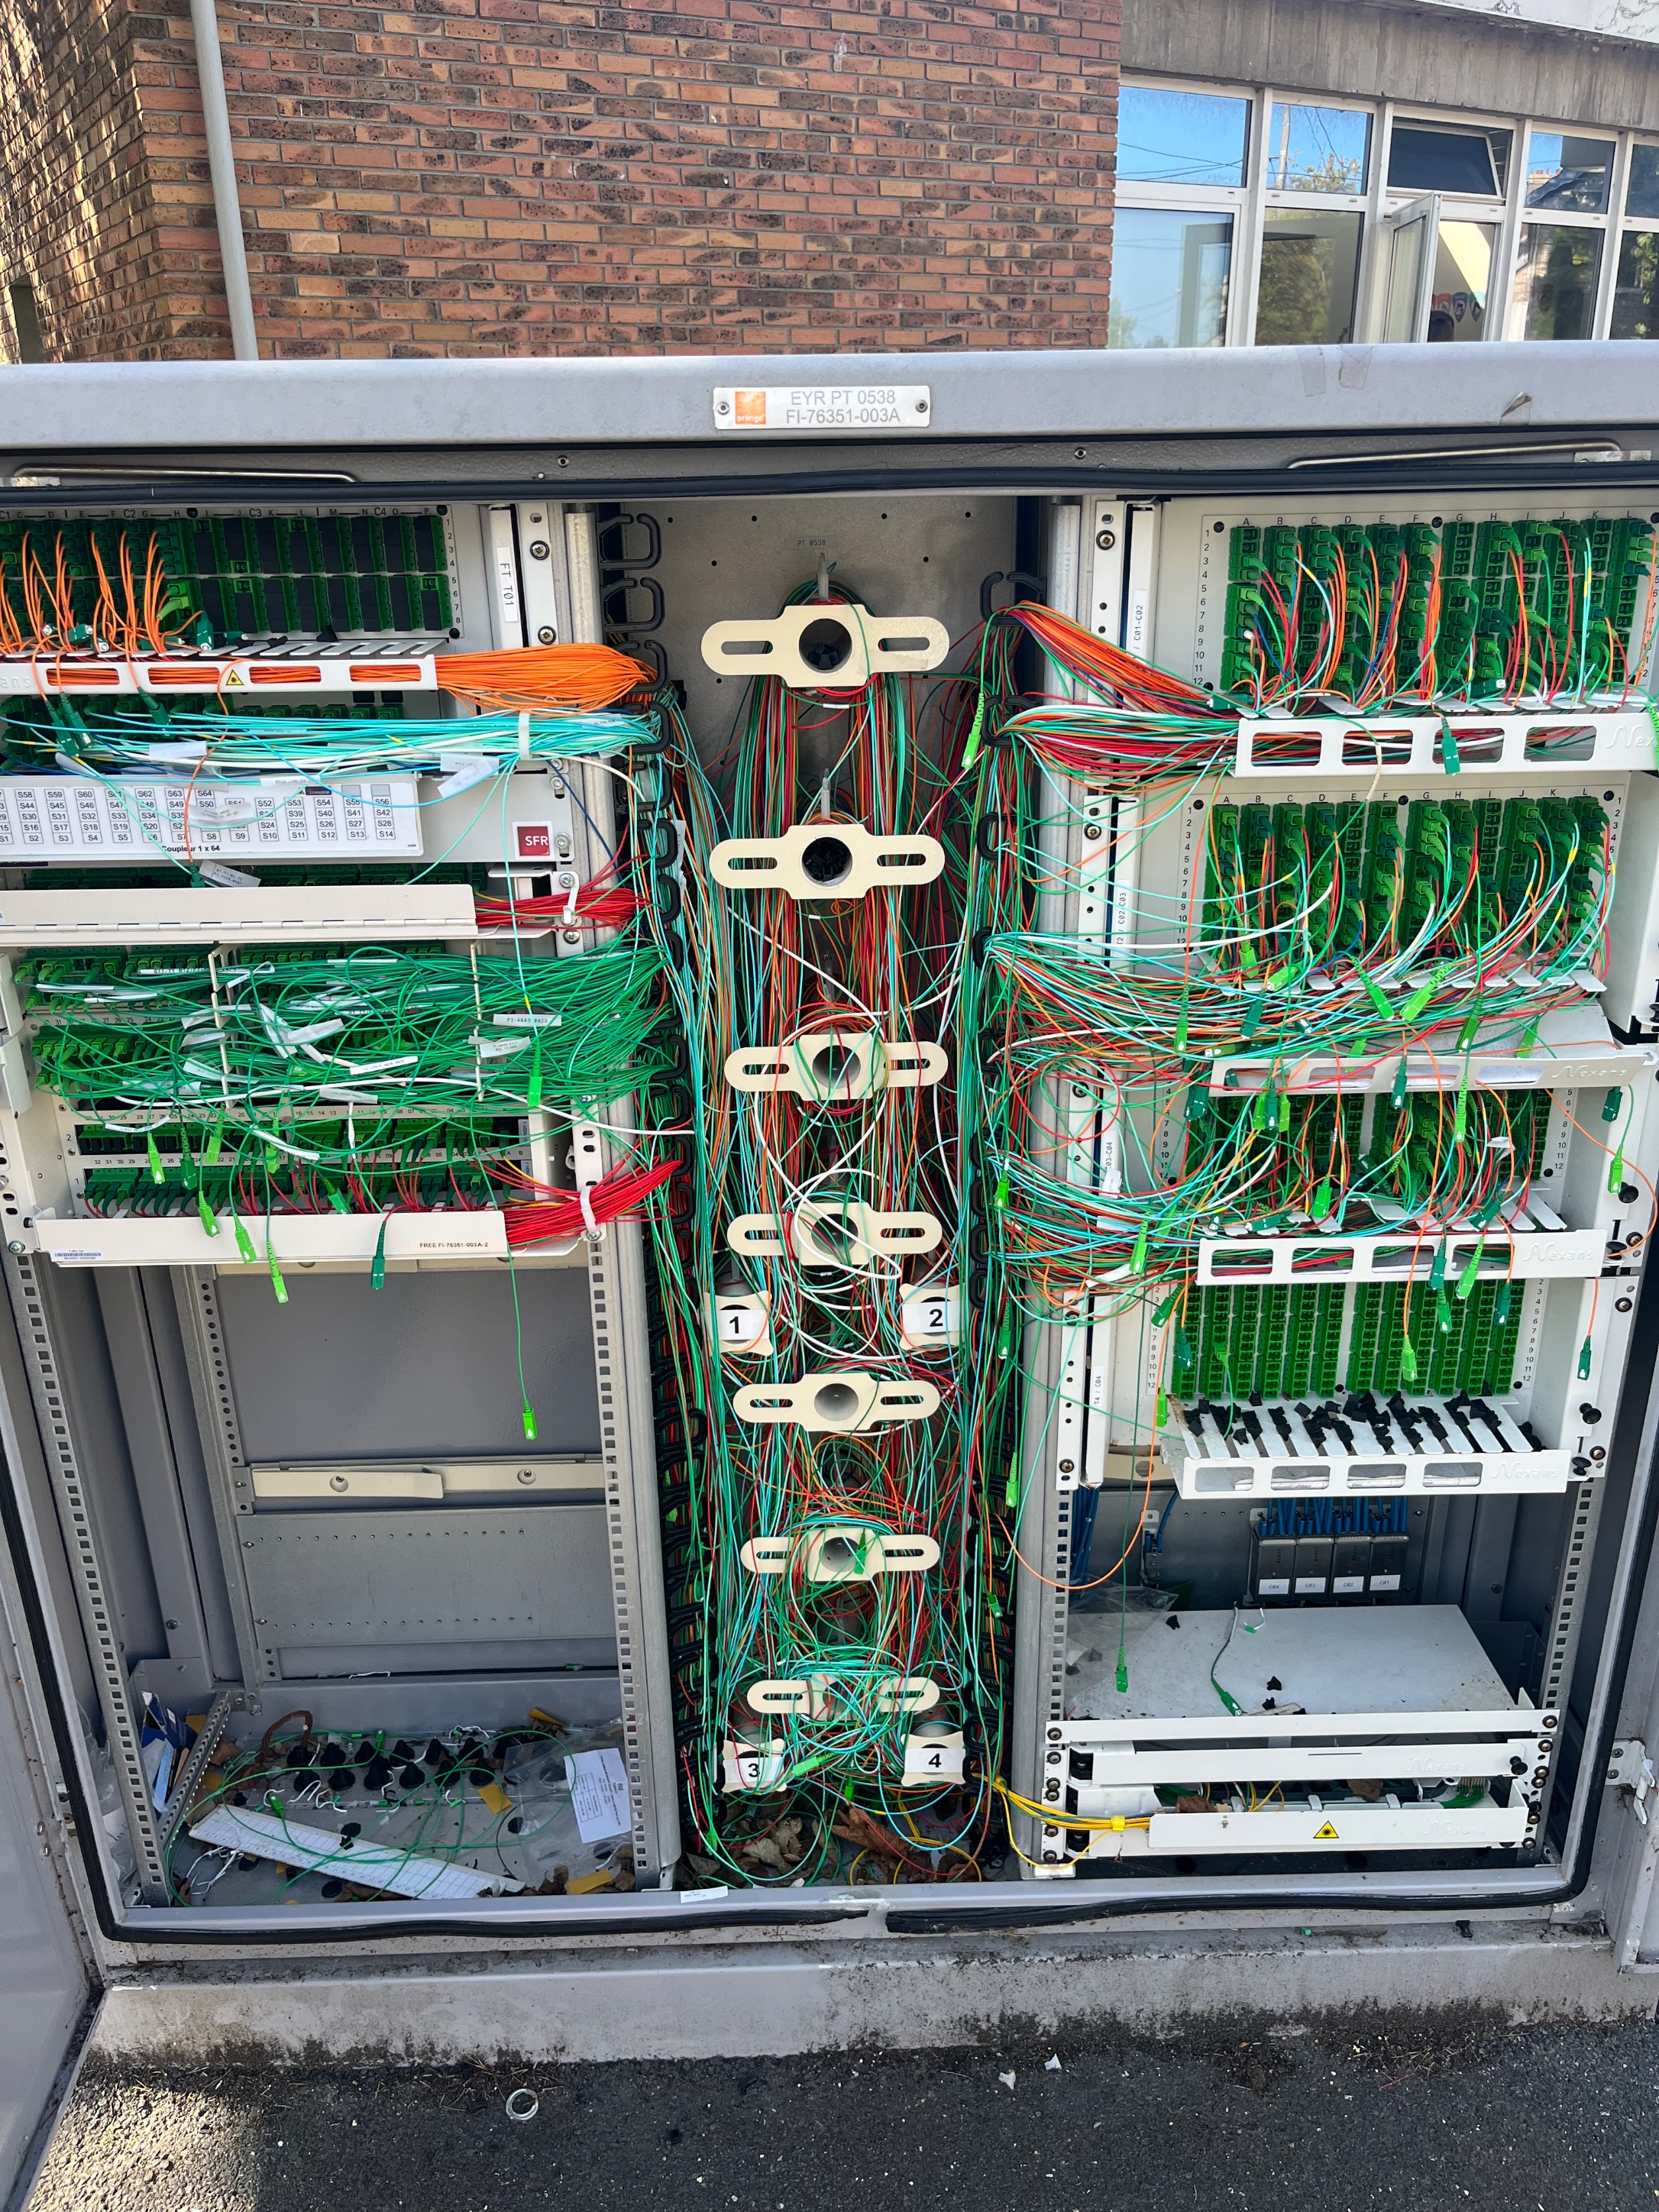
\includegraphics[width=\linewidth]{images/false_positif/5173534_2.jpg}
        \caption{Example of a false alarm - 2}
    \end{subfigure}
\end{figure}

In this case, these 2 images have been captured on different days of the year. It could be noticed when to notice the lighting of the image under the left PM door. In the second image, there was sunlight in the ground around the PM and the first, there was not.

\begin{figure}[H]
    \centering
    \begin{subfigure}{0.4\textwidth}
        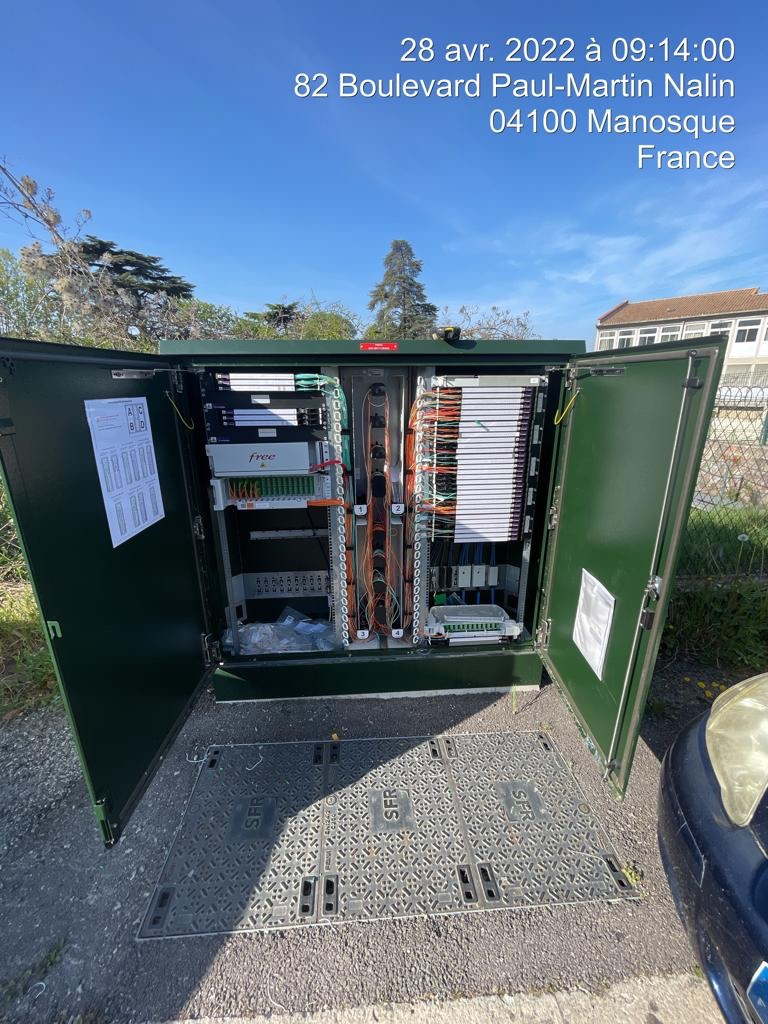
\includegraphics[width=\linewidth]{images/false_positif/f3_1.jpg}
        \caption{Example of a false alarm - 1}
    \end{subfigure}
    \begin{subfigure}{0.4\textwidth}
        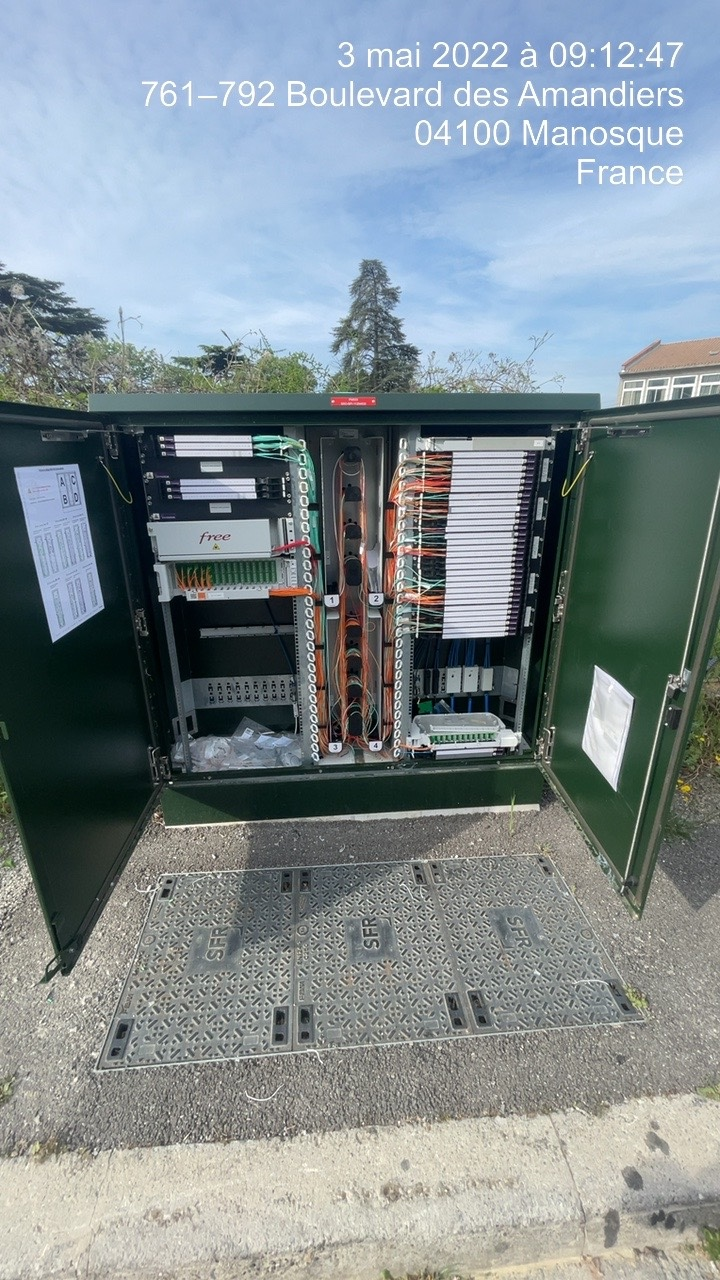
\includegraphics[width=\linewidth]{images/false_positif/f3_2.jpg}
        \caption{Example of a false alarm - 2}
    \end{subfigure}
\end{figure}

In this case, the sky was different because it was on different days. There was also a head of a car on the right of the image in the second image.

\subsection{Method}

This is the overview of the method to compare the similarity between images. The input is the combination of 2 images. The image that is already exists on the database called the \textbf{map} image. The image that it is recently appears that we need to check if forgery is called the \textbf{template} image.

\begin{figure}[H]
    \centering
    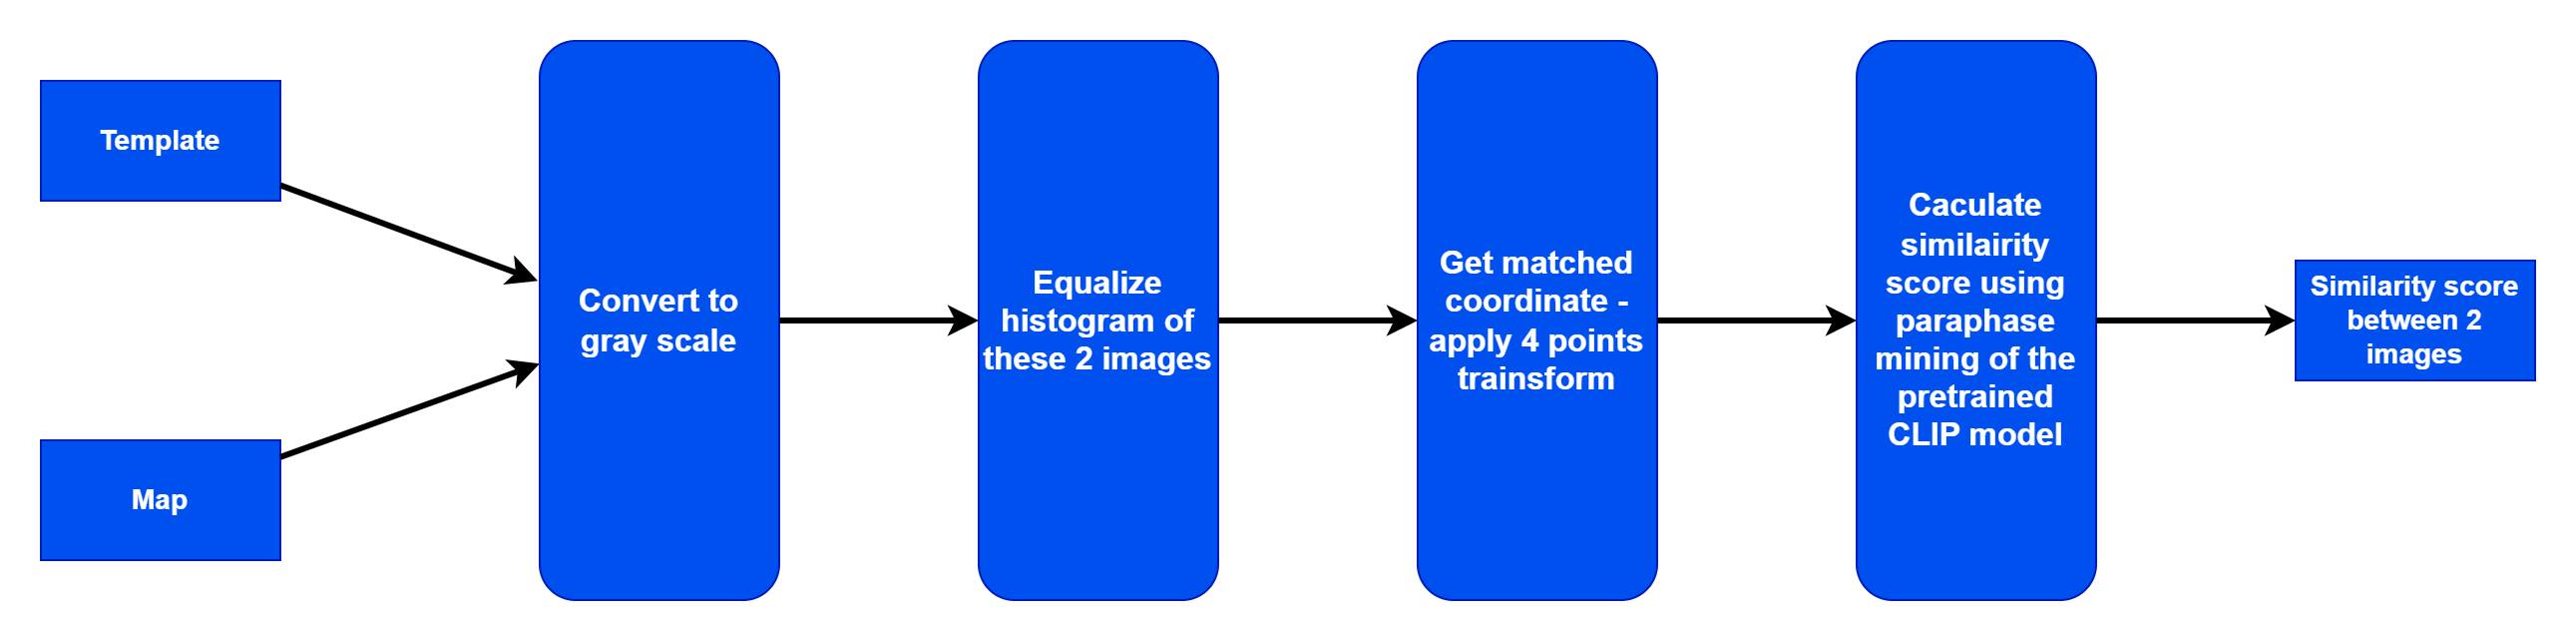
\includegraphics[width=1\textwidth]{images/pm_describe.drawio.png}
    \caption{Overall architecture of the forgery detection system}
    \label{fig:altice_campus}
\end{figure}

\begin{itemize}
    \item \textbf{Convert to grayscale}
    
First, to deal with the problems of color shifting in some of the forgery cases, we need to convert both the map and the template to grayscale images.

    \item \textbf{Equalize histogram}

Even the shift of the lighting image is also important to this task. I use the OpenCV\cite{opencv_library} equalizeHist() function to equalize the histogram of the image before proceeding to the next image.

    \item \textbf{Four points transform}

The scale-invariant feature transform (SIFT)\cite{lowe1999object} is a computer vision algorithm to detect, describe, and match local features in images. Applications include object recognition, robotic mapping and navigation, image stitching, 3D modeling, gesture recognition, video tracking, individual identification of wildlife and match moving.

In this case, I use SIFT to detect the common feature between 2 images and then map the common feature between them. Once the number of matched features exceeds the set threshold, we could use OpenCV homography to correct the point of view of the template to the map.

\begin{figure}[H]
    \centering
    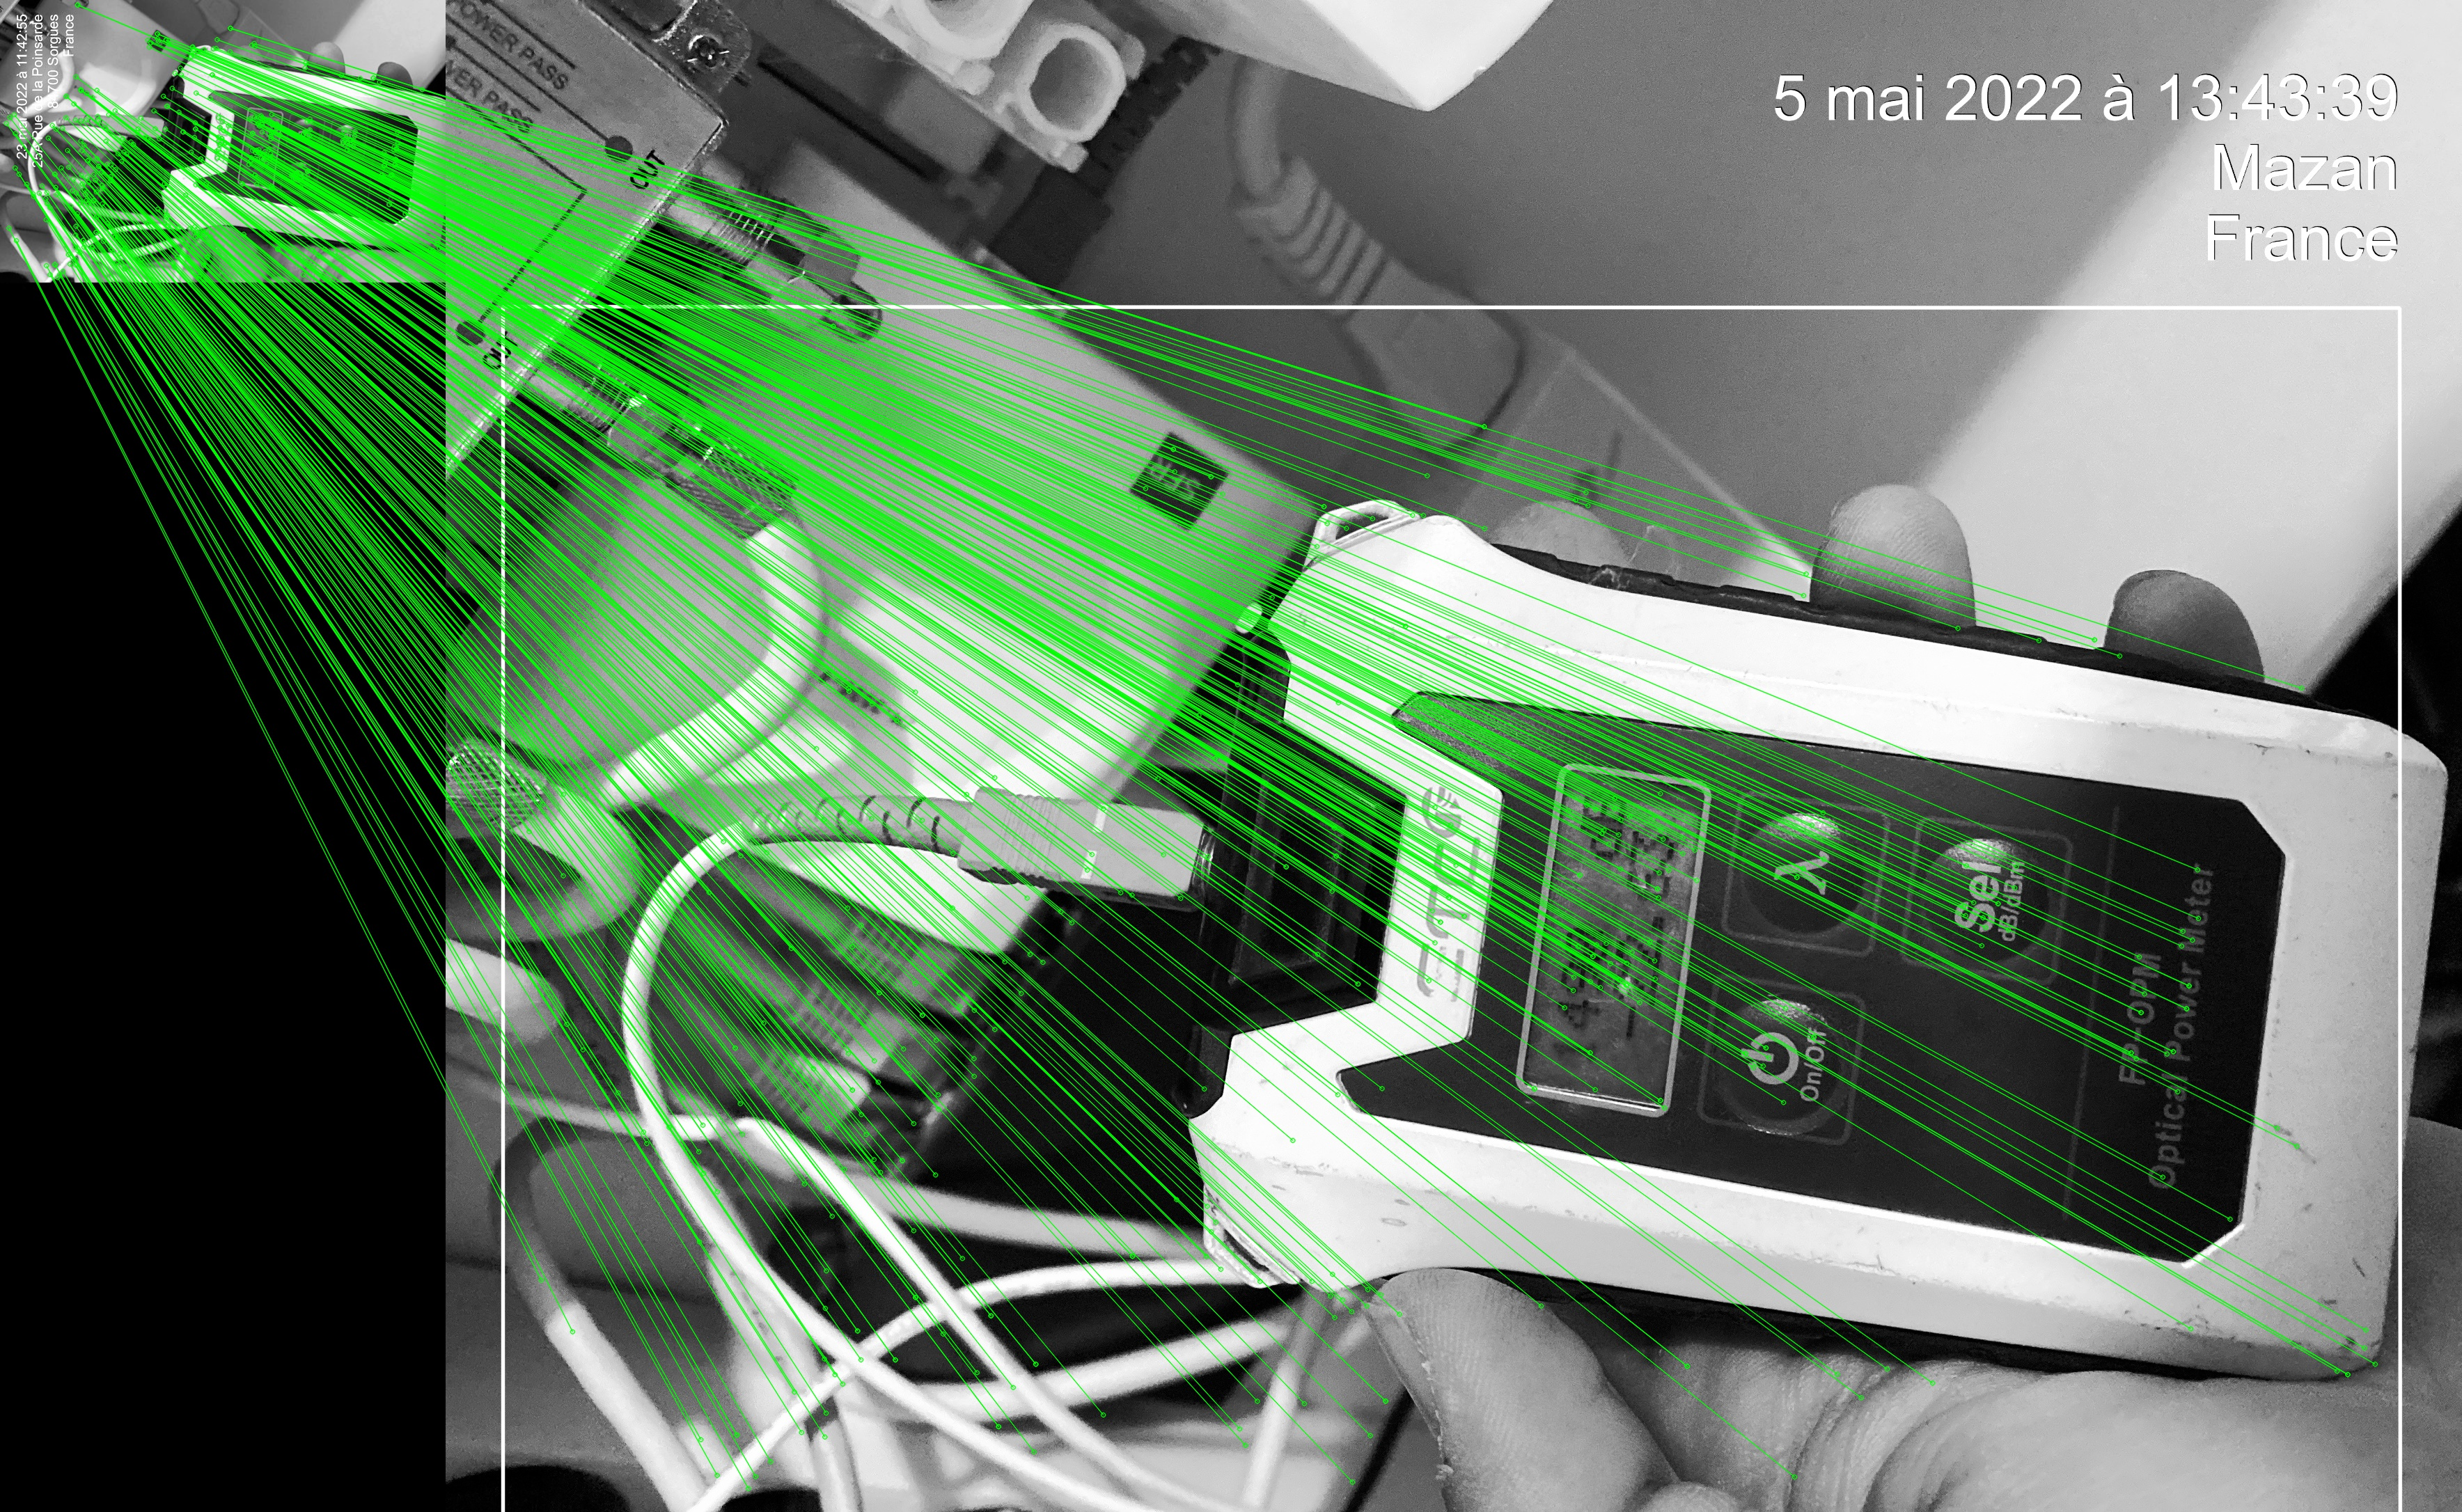
\includegraphics[width=0.8\textwidth]{images/example_front.jpg}
    \caption{Using SIFT and homography to find the coordinate from the template to the map}
    \label{fig:sift}
\end{figure}

The next critical step is to transform the four-point coordinates of the image into a rectangle, like a bird's eye view. We need to do this in the case of detecting images that have been slightly rotated.
    
    \item \textbf{Represent the images to vectors using Contrastive Language-Image Pre-Training (CLIP) model}

In this step, the template has been cropped and transformed to have the same view as the map. So we will be able to avoid retouched elements before we use CLIP\cite{pmlr-v139-radford21a} to calculate the representation vector of the image, thus hoping false alarm cases like the example in 3.1.1 do not affect the representation.
    
\end{itemize}

\subsection{Results}

Due to the lack of labels and lack of true positive cases, I need to create more of the dataset myself by capturing images inside the SFR campus. I captured 2 images of the same place at different times and different angles and created a forgery myself using one of the images with the same forgery techniques that technicians use.

\begin{itemize}
    \item image 1: Original image
    \item image 2: Capture the same place but at a different time and angle
    \item image 1 forgery: a modified version of image 1
\end{itemize}

The dataset used to test this method has been carefully labeled manually, both captured by myself and detected real cases. The score is from 0\% to 100\%, with the higher the score, the most lookalike between 2 images and 100\% is identical.

\begin{figure}[H]
    \centering
    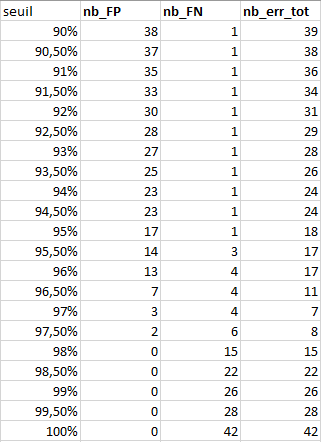
\includegraphics[width=0.5\textwidth]{images/cas_2_confusion_matrix.png}
    \caption{Table of the number of errors by choosing different thresholds of similarity}
    \label{fig:clip_threshold}
\end{figure}


\begin{table}[H]
\centering
\captionof{table}{Threshold table description} \label{tab:description_threshold} 
\begin{tabular}{|l|l|}
\hline
\textbf{column name}  & \textbf{description}              \\ \hline
seuil        & similarity threshold     \\ \hline
nb\_FP       & number of false positive \\ \hline
nb\_FN       & number of false negative \\ \hline
nb\_err\_tot & total number of error    \\ \hline
\end{tabular}
\end{table}

\begin{figure}[H]
    \centering
    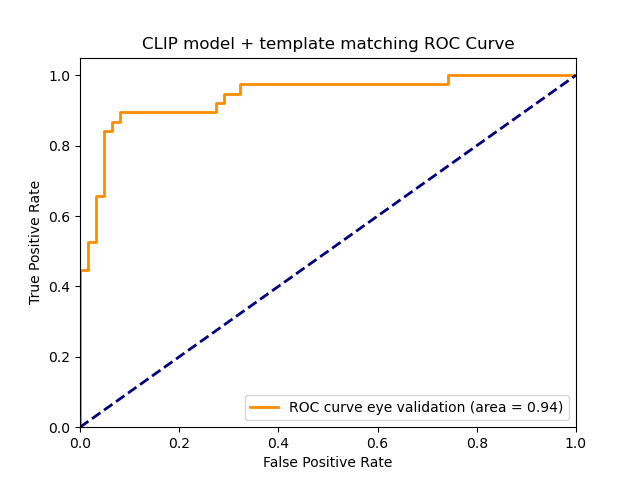
\includegraphics[width=0.8\textwidth]{images/cas_1_roc-curve.png}
    \caption{ROC curve of the method}
    \label{fig:clip_roc-curve}
\end{figure}

As the results show, the best threshold to choose is around 97\% of similarity between the template and the map. Above this score, it is usually forgery cases and below this is false alarm cases.

\section{Research the feasibility of moving the team's infrastructure to the Google Cloud}

\subsection{Example of needed cases}

SFR is an operator in France responsible for managing and maintaining a network of mobile signal towers. Your goal is to ensure uninterrupted mobile signal and internet services for your customers while minimizing downtime and troubleshooting issues efficiently.

Ensuring consistent network performance is challenging due to the complexity of signal tower operations and the potential for various issues such as hardware failures, signal interference, and congestion. We want to implement a system that can detect anomalies in real-time and help us address them before they impact customer experience.

\subsection{Use case of VertexAI}

\begin{itemize}
    \item \textbf{Data Collection and Integration:}
    
    Data is collected from multiple sources within the network, including signal strength measurements, network traffic data, tower hardware status, and historical performance data.
    \item \textbf{Model Development:}

    Machine learning models for anomaly detection are developed using Vertex AI's capabilities. These models are trained on historical data to learn normal patterns of network behavior.

    \item \textbf{Real-time Anomaly Detection:}

    Deployed models continuously monitor incoming data from signal towers in real-time.
    Deviations from expected patterns trigger alerts, notifying network operators of potential anomalies.

    \item \textbf{Alert Prioritization and Response:}

    Generated alerts are prioritized based on severity and potential impact on network performance. Vertex AI's insights assist in identifying root causes and appropriate responses.

    \item \textbf{Continuous Improvement:}

    Feedback loops are established to refine models based on accuracy and response effectiveness. Collaboration with data scientists fine-tune models for improved anomaly detection.

    \item \textbf{Performance Monitoring:}

    Vertex AI's visualization tools track the overall performance of the anomaly detection system. Key metrics, including detected anomalies, false positives, and response times, are monitored.
\end{itemize}




\section{Apply machine learning techniques on call log from SFR's call center}

The below diagram shows the overall architecture of the system. We want to try to benefit the representation of the language model in this use case of finding the topics in the corpus of the company's call center.

\begin{figure}[H]
    \centering
    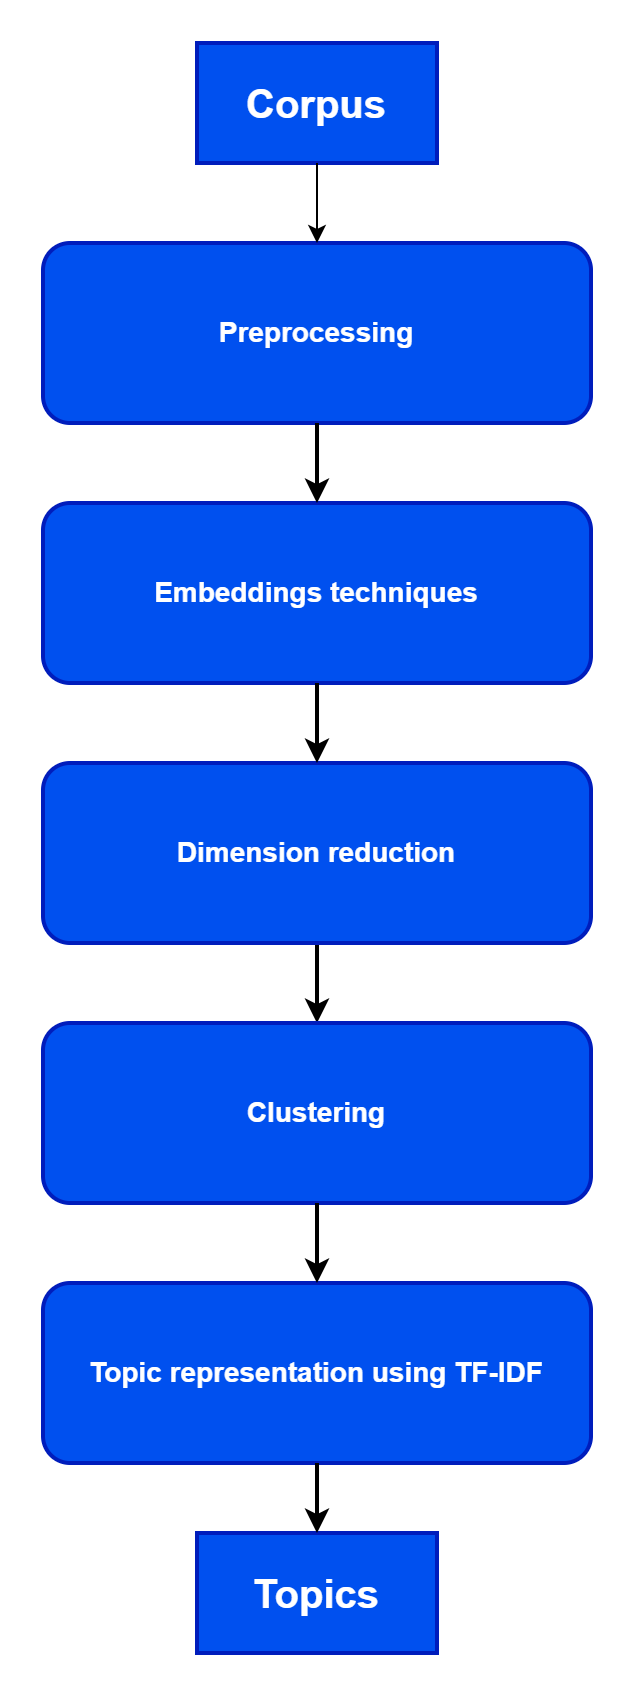
\includegraphics[width=0.4\textwidth]{images/describe_nlp.drawio.png}
    \caption{Algorithm description}
    \label{fig:nlp_describe}
\end{figure}

The process starts with preprocessing, which turns the given dataset into the form that is needed for the embedding techniques. Some soft clean is also applied to the corpus before translating the sentence into vectors. After we have the desired corpus, it will be represented as a vector in a fined vector space with the help of a sentence transformer. The dimension reduction techniques are then applied, and we use the output of the process as data points to do the main task of clustering. After that, we use a special version of TF-IDF to find the most significant word of each found topic.

This project will be kept as the topic for the memoir, I will go into further detail in the memoir section. This part will introduce briefly the overall architecture.

The output of this project is the list of significant words and the input is the new conversation with the customer that was also introduced to the system.

\begin{figure}[H]
    \centering
    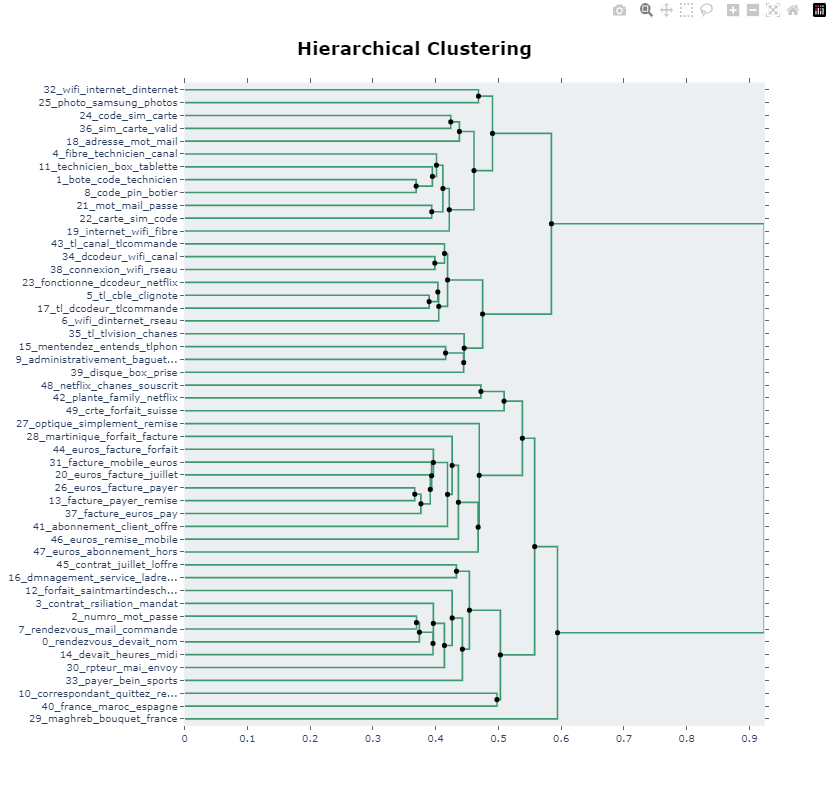
\includegraphics[width=1\textwidth]{images/results/cam/hierachy_pca_tree.png}
    \caption{One of the results using hierarchy clustering and PCA}
    \label{fig:hierachy_pca}
\end{figure}

\chapter{Assessment and proposals}

\startcontents[chapters]
\printmyminitoc{
}

\section{Fiber distribution point images processing}

The previous system with image fingerprints method can filter out 90\% of the false cases, only 10\% need to pass to the new system for deeper inspection. With the accuracy of the new method is over 90\% with the images that bypass the fingerprint method, Now the accuracy of the combination of these 2 systems together is 99\%, and it is already deployed in the production environment. 

However, this method still has a drawback. The time to proceed with a case, from input to output is the similarity score is considered slower than the fingerprint method. This is also the reason why we don't replace it completely but set it as an additional section<

\section{Research the feasibility of moving the team's infrastructure to the Google Cloud}

With the undeniable advantages of moving to Google Cloud compared to the current local server and workflow, we have the opportunity to revolutionize the way we manage our IT resources and drive significant improvements across various aspects of our organization. It could take some effort to build the system in the beginning but the benefit after it is huge. After my research, the company decided to start the process of moving to the cloud starting in September 2023. I will depart before the transition but I hope the transition could facilitate the workflow in the future, and at the same time increase the stability of the production environment that we currently have.

\section{Apply machine learning techniques on call log from SFR's call center}

We can see that in the tree of hierarchy clustering techniques, the most significant word of each topic is very promising. This method can cluster use cases in each small topic, with the cluster of technical problems, or the cluster of invoices, etc. being very well separated. We can also see that the relationship between clusters that are not so far from each other, for example, the invoice topics is close to the termination service. The termination of the customers is usually because they are not happy with the current payment problem.

This method still has some drawbacks. With one conversation, it could only be classified as one topic. However, in reality, One conversation could contain multiple topics at the same time. The customer could call the call center for multiple reasons or multiple problems. This point should be a point to focus on and research in the future of this project.
\chapter{Conclusion}

\startcontents[chapters]
\printmyminitoc{
}

The apprenticeship offers a valuable opportunity for me to improve my skills, and a chance to apply what I have learned over the courses at the university on real projects. Equally significant is the examination of the result at the end of this journey — what the experience has brought to me and, conversely, what I have contributed to the company.

\section{Knowledge acquired after the apprenticeship}

Through the apprenticeship, I've acquired a wealth of valuable knowledge an
d insights. I've honed my skills in data collection, analysis, and interpretation, especially in the context of customer interactions. Additionally, I've applied and learned a lot of things from multiple technologies such as NLP, working with cloud and computer vision. These experiences have not only expanded my technical expertise but have also deepened my understanding of the intricacies of the telecommunications industry and the significance of customer-centric strategies. Not only that, it is also important for me to acquire the necessary soft skills, teamwork skills, and communication skills.

Overall, the apprenticeship has equipped me with a diverse skill set and a practical perspective that I can apply to future endeavors.


\section{Contributions}

In the part of contributions to the company, my role as an apprentice data scientist apprentice at SFR entailed a range of responsibilities. I actively engaged in data collection, analysis, and the application of advanced techniques to extract meaningful insights from complex datasets. This process was necessary in informing strategic decisions, optimizing operational processes, and enhancing customer experiences. Furthermore, my collaborative interactions with cross-functional teams facilitated the alignment of data-driven insights with business objectives and promoted an environment of better decision-making. 

I hope my contribution will help the business for SFR not only resolve current problems and business, but also it could use the research about the cloud in the near future as planned.





\part{Master's thesis}
\chapter{Introduction}

\startcontents[chapters]
% \printmyminitoc{

% }

 Ensuring customer satisfaction stands as one of the most important goals for enterprises across industries. Customer satisfaction is a term frequently used in marketing. It is a measure of how products and services supplied by a company meet or surpass customer expectations. Customer satisfaction is defined as "the number of customers, or percentage of total customers, whose reported experience with a firm, its products, or its services (ratings) exceeds specified satisfaction goals."\cite{cus_sas} Customers play an important role and are essential in keeping a product or service relevant, so it is, therefore, in the best interest of the business to ensure customer satisfaction and build customer loyalty. 

\begin{figure}[H]
    \centering
    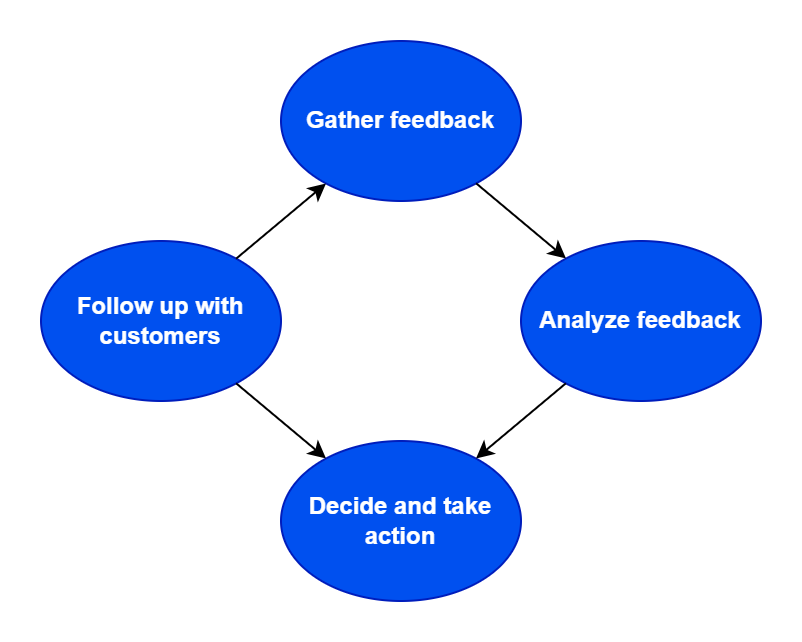
\includegraphics[width=0.7\textwidth]{images/customer-sastifaction.drawio.png}
    \caption{Customer satisfaction loop}
    \label{fig:cus_satis}
\end{figure}

With fierce competition in today's market, the collection and analysis of invaluable data derived from customer interactions is the key to improving companies' competitive advantage. Analysis of customer calls to the call center by using NLP techniques to distill meaning from these interactions and extract actionable insights is also one of the missions that the company takes place to improve customer relationships and heighten service quality.

To achieve this objective, I use NLP techniques to cluster the recorded phone calls of the customer with the SFR call center. Central to this approach is the utilization of CamemBERT\cite{martin2020camembert}—a specialized French language model and variant of the RoBERTa\cite{liu2019roberta} architecture. CamemBERT is leveraged to transform the linguistic essence of each sentence into a vector within a vector space. These vectors serve as a representation of the meaning of each sentence. After that, I will apply some clustering techniques in these transformed vectors, thus discovering the most important words of each cluster by using TF-IDF, a technique to extract pivotal keywords, and the most representative documents closely aligned with centroids.

The objective is to use the most significant word of each topic as a suggestion for the call team, who need to determine the topic of calls manually. By suggesting the words and the topics for the team, it could be easier to label topics for the call, as well as the labeling process will be more accurate and suggest the labelers to labels that he or she does not have enough time to describe a conversation and select all relevant tags fully.
\chapter{Theoretical background and materials}

\startcontents[chapters]
\printmyminitoc{
    
}



\section{Theoretical background}

\subsection{Topic modeling}

In NLP, topic modeling is a type of model that finds the overall topics that are shown in given documents, usually in the form of a corpus.

This method uses the statistic of the frequency of the words that appear in documents to identify the common between documents without knowing the predefined label and training data. For example in our case of a call center of an operator, a topic modeling algorithm could find whether the topic of documents are invoices, bills, telephones, or fiber based on their contents. Latent semantic analysis (LSA)\cite{deerwester-indexing-1990} latent Dirichlet analysis (LDA)\cite{944937} or Non-Negative Matrix Factorization (NMF)\cite{conf/nips/LeeS00} are some of the topic modeling methods that analyze large text files to categorize topics, provide valuable insights, and support better decision-making.

Topic modeling methods are also considered probabilistic topic models, which refer to statistical algorithms for discovering the latent semantic structures of an extensive text body. Nowadays, the amount of information that we receive each day is simply out of the ability of process of humans. This technique can help to organize and offer insights for us to understand the large amount of data that we encounter. From text-mining at first, topic modeling methods nowadays could also help to detect patterns in data such as genetic information, images, and networks. It also has applications in bioinformatics and computer vision.

\subsection{Word embedding}

In NLP, a word embedding is a representation of a word in the form of a vector in a vector space. The embedding is used in text analysis. Typically, the representation is a real-valued vector that encodes the meaning of the word in such a way that words that are closer in the vector space are expected to be similar in meaning. Word embeddings can be obtained using language modeling and feature learning techniques, where words or phrases from the vocabulary are mapped to vectors of real numbers.

Methods to generate this mapping include neural networks, dimensionality reduction on the word co-occurrence matrix, probabilistic models, explainable knowledge base method, and explicit representation in terms of the context in which words appear.

Word and phrase embeddings, when used as the input representation, have been proven to boost the performance in multiple NLP tasks such as syntactic parsing and sentiment analysis.

\subsection{Our way to find topics in a given corpus}

To reveal underlying common topics of a corpus, topic models have been shown to be an effective tool. Convention techniques like Latent Dirichlet Allocation (LDA)\cite{944937} or Non-Negative Matrix Factorization (NMF)\cite{conf/nips/LeeS00} describe corpus as a set of words and represent each document as a mixture of topics.

The big drawbacks of this method are they could lose the meaning and relation between words when it forms a bag-of-words, and it only uses the count of the number of words that appear in a document but does not account for the relationship and the context of words with each other inside a document.

For example, the word "bank", is the same in the river bank, and the bank is a place to store and borrow money if we apply Bag-of-Words\cite{bagofwords} and use LDA over it. However, if we apply a language model, the model could distinguish the differences between these 2 words "bank". They have the same representation but have different meanings due to different surrounding contexts.

We want to apply the advantage of language models to find the topics in a corpus.



\section{Materials}

\subsection{Tools}

\begin{figure}[H]
    \centering
    
\includegraphics[width=0.3\textwidth]{images/python.png}
    % \caption{Python}
    \label{fig:python_logo}
\end{figure}

This project was done by using Python. Python is one of the most popular programming languages in the field of data science, and for good reason. It offers numerous advantages that make it well-suited for data analysis, machine learning, and other data science tasks. Some of the key advantages of using Python in data science include:

\begin{itemize}
    \item \textbf{Rich Ecosystem of Libraries:} Python has a vast collection of libraries and frameworks specifically designed for data science tasks. Libraries like Numpy\cite{harris2020array}, pandas\cite{mckinney-proc-scipy-2010}, Matplotlib\cite{Hunter:2007}, Seaborn, and scikit-learn\cite{scikit-learn} provide powerful tools for data manipulation, analysis, visualization, and machine learning.
    \item \textbf{Versatility:}  Python is a general-purpose programming language, meaning that it's not limited to data science tasks. This versatility allows data scientists to integrate their work with other areas of development, creating end-to-end solutions. The extension of this project is not only about finding the topic of the dataset but also about building an end-to-end system for the usage of agents.
    \item \textbf{Jupyter Notebooks:}  Jupyter Notebooks\cite{Kluyver2016jupyter} provide an interactive and shareable environment for data analysis. They allow you to combine code, visualizations, and explanatory text in a single document, making it easy to document your work and share insights with others.
    \item \textbf{Data Visualization:}  Python offers several powerful visualization libraries, such as Matplotlib and Seaborn, that allow you to create informative and aesthetically pleasing graphs and charts to convey your findings effectively.
\end{itemize}

Besides common Python libraries that are used to process the data, for example, Pandas, Numpy, Scikit-learn, etc., it is necessary to use some of the famous libraries in the NLP field. Also, it is not recommended to do the preprocessing on a language model like BERT, but I do use Natural Language Toolkit (NLTK)\cite{bird2009natural} to do some light cleaning due to the original dataset containing a lot of noise. 

2 language models applied in this project are CamemBERT\cite{martin2020camembert} and MiniLMv2\cite{wang2021minilmv2} through the Sentence Transformer library. It helped to embed conversations and we represented both of them to find the best technique for our use case.

Scikit-learn is used to deploy clustering and dimension reduction techniques.

\subsection{Datasets}

The data that I use in this project is the transcribed call logs from the SFR customer care center database. In SFR, we use Apache Impala and Apache Hive to store information. However, to have permission to access such sensitive information, requires a special permit.

At first, I intended to use every call from June 2022, but it is proven that processing all of such huge data is considered too ambitious, with more than 7 billion words. My final dataset contains 100 million words from the first of June 2023 to the present.

The raw data table has a lot of information, but in the end, we only consider these columns.

\begin{table}[H]
\centering
\captionof{table}{Database description} \label{tab:description_database} 
\begin{tabular}{|lp{10cm}|lp{10cm}|}
\hline
\textbf{column name}  & \textbf{description}                                                                  \\ \hline
contact\_id           & ID of the conversation                                                                \\ \hline
transcript\_speaker   & 2 channels exist. Channel 1 is for our agent, and channel 2 is for the customer \\ \hline
transcript\_word      & Word of the transcript                                                                \\ \hline
transcript\_starttime & Time of each word when it is being spoken                                             \\ \hline
\end{tabular}
\end{table}

Each row in the table contains only one word, and the location is defined as the contact\_id, which is the id of the conversation and the transcript start time, with the beginning of the conversation as the second 0.

\begin{figure}[H]
    \centering
    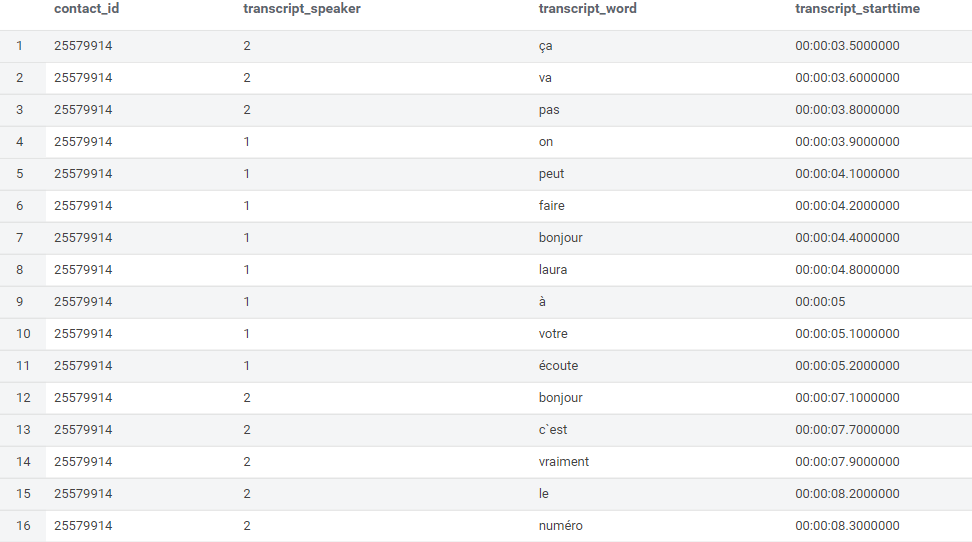
\includegraphics[width=1\textwidth]{images/db_example.png}
    \caption{Example of the format of the raw dataset}
    \label{fig:raw_dataset}
\end{figure}







\chapter{Methods}

\startcontents[chapters]
\printmyminitoc{
}


\section{Overview of the method used}



The below diagram shows the overall architecture of the system. We want to try to benefit the representation of the language model in this use case of finding the topics in the corpus of the company's call center.

\begin{figure}[H]
    \centering
    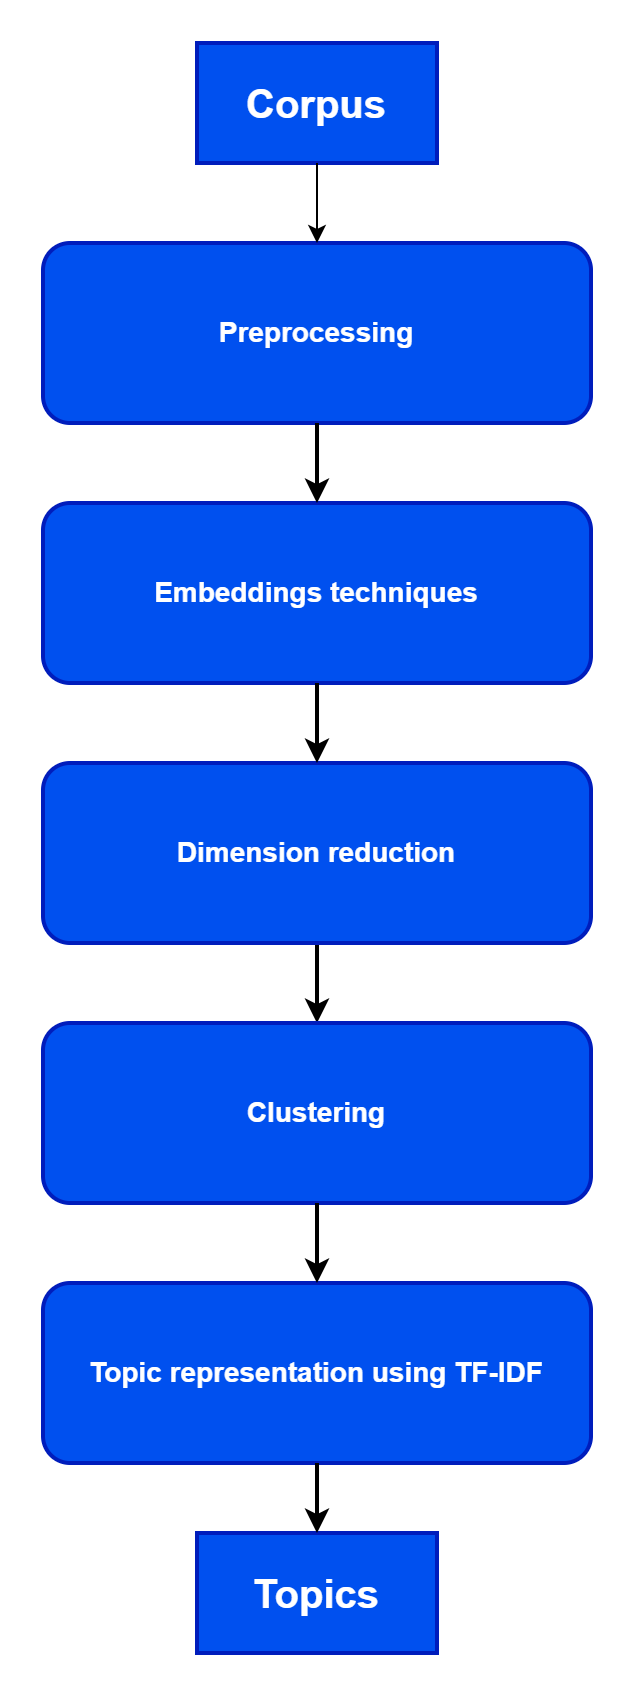
\includegraphics[width=0.4\textwidth]{images/describe_nlp.drawio.png}
    \caption{Algorithm description}
    \label{fig:nlp_describe}
\end{figure}

The process starts with preprocessing, which turns the given dataset into the form that is needed for the embedding techniques. Some soft clean is also applied to the corpus before translating the sentence into vectors. After we have the desired corpus, it will be represented as a vector in a fined vector space with the help of a sentence transformer. The dimension reduction techniques are then applied, and we use the output of the process as data points to do the main task of clustering. After that, we use a special version of TF-IDF to find the most significant word of each found topic.

\section{Preprocessing}

As you can see in the example of the raw database in section 7.3, The current data is stored in the Impala database. To begin to work with the data, I created a SQL script to pull the most recent transcription from the database and store it as a Pandas data frame, in the form of a pickle file. We will only need to pull the column that contains the value data.

\begin{table}[H]
\centering
\captionof{table}{Database description} \label{tab:description_database} 
\begin{tabular}{|lp{10cm}|lp{10cm}|}
\hline
\textbf{column name}  & \textbf{description}                                                                  \\ \hline
contact\_id           & ID of the conversation                                                                \\ \hline
transcript\_speaker   & 2 channels exist. Channel 1 is for our agent, and channel 2 is for the customer \\ \hline
transcript\_word      & Word of the transcript                                                                \\ \hline
transcript\_starttime & Time of each word when it is being spoken                                             \\ \hline
\end{tabular}
\end{table}

The data needs to be sorted in order. This is because when the words are being stored, it is not necessary in the order of the speaker. Only when we sort by transcript\_starttime and transcript\_speaker, we will have a correct order of the conversation. It is also important that the newest data is prioritized, which means when the data is selected, the partdate, which is the date that these pieces of information are recorded also needs to be sorted in ascending order.

After the data is in good order, The data is merged into conversations, with each row should have the same contact\_id. Here is the result of the process after the merge.

\begin{figure}[H]
    \centering
    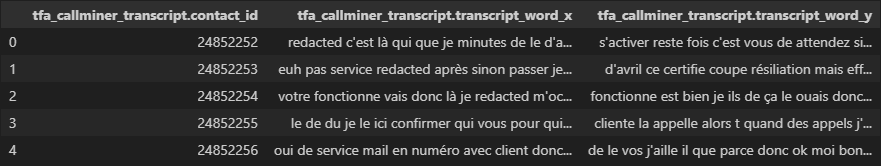
\includegraphics[width=1\textwidth]{images/dataset_merged_example.png}
    \caption{Dataset after the merge into big conversation}
    \label{fig:dataset_merge}
\end{figure}

It is not recommended to do the preprocessing with the corpus before feeding into a language model. However, the call here is a log of a speaking conversation. Speaking is not the same as writing, and we tend to put a lot of filler words to avoid emptiness while speaking. Therefore, before going to the next step of embedding the documents, These filler words should be removed to avoid confusion in the language model.

The French filler words vary, but 20\% of them can speak more than 90\% of the time. I only removed the word that I saw appear too many times.

\begin{lstlisting}[language=Python]
filler_word = ['redacted', 'bonjour', 'oui', 'monsieur', 'madame', 'ben', 'quelque', 'moment', 'justement', 'euh', 'non', 'hein', 'collègue', 'hein', 'allô', 'ah', 'alors', 'voilà', 'bah']
\end{lstlisting}

\section{Document embeddings}

We start by converting the current document that we just cleaned into numerical representation, and we will use a sentence transformer to do it.

A Sentence Transformer is a type of model designed to convert sentences or short text snippets into fixed-length vector representations, and we call it embeddings. These embeddings capture the semantic meaning and context of the input sentences, allowing for meaningful comparisons, similarity calculations, and downstream tasks in NLP.

Unlike traditional word embeddings, which generate vector representations for individual words, sentence transformers focus on creating embeddings for entire sentences. This is particularly useful when the meaning of a sentence is influenced by the arrangement and interaction of its words.

Sentence transformers are typically built using transformer architecture, which has proven highly effective in capturing contextual information and semantic relationships in text. The key innovation lies in how these models are fine-tuned to create sentence embeddings. During training, the model learns to generate embeddings in such a way that sentences with similar meanings are closer together in the embedding space, while sentences with different meanings are farther apart. Therefore, the application of clustering techniques for these embeddings is well-founded.

\subsection{CamemBERT}

Camembert is a state-of-the-art NLP model based on Roberta. It is part of the transformer-based architecture family, which has shown remarkable success in various NLP tasks. Camembert is specifically designed for understanding and generating human language text. It draws its name from the famous French cheese, just like the BERT model it is built upon.

Camembert is pre-trained on large amounts of text data to learn the underlying patterns and structures of language. This pre-training enables the model to understand the context, semantics, and relationships between words in a sentence. The key innovation of Camembert lies in its ability to understand sentences in French. Unlike Roberta that were trained in English, Camembert is trained in a French corpus.

In this case, we will use a specific version of CamemBERT, which is sentence transformer camemBERT. The model is Fine-tuned using pre-trained Facebook camembert-large and Siamese BERT-Networks with 'sentences-transformers' on dataset stsb.

\subsection{miniLMv2}

MiniLM is a compact and efficient language model developed by Microsoft Research. It's designed to offer a balance between model size and performance, making it well-suited for various natural language processing tasks. MiniLM is built upon the transformer architecture, which has proven to be highly effective for tasks like text generation, translation, and understanding.

One of the key features of MiniLM is its smaller size compared to its larger counterparts, such as BERT or RoBERTa. Despite its reduced size, MiniLM aims to retain competitive performance on a range of language-related tasks. This is achieved through careful optimization of the model architecture, training process, and compression techniques.

This architecture was updated in mid-2021 and has even better results and performance. In this project, a multilingual version of MiniLMv2 will be applied and we will have some comparison with CamemBERT. We will use the sentence transformer fine-tuned version of this model instead of the original one

\section{Dimension reduction}


\subsection{PCA}

Principal Component Analysis (PCA) is a traditional and widely used dimensionality reduction technique in the field of data analysis and machine learning. Its primary goal is to simplify the complexity of high-dimensional data while preserving as much relevant information as possible. PCA achieves this by transforming the original data into a new coordinate system where the dimensions, known as principal components, are orthogonal (uncorrelated) and capture the maximum variance in the data. 

Since the output of the sentence transformer still contains too many features, It is advised to use some techniques of dimensional reduction to reduce the number of features.

However, PCA still has some drawbacks:

\begin{itemize}
    \item Loss of Interpretability: The principal components are linear combinations of original features, which can make them difficult to interpret in terms of the original domain.
    \item Linearity Assumption: PCA assumes that the underlying relationships in the data are linear. It may not capture complex nonlinear patterns.
    \item Dependence on Variance: PCA focuses on variance, which might not be the most suitable criterion for all types of data or applications.
\end{itemize}


\subsection{UMAP}

UMAP (Uniform Manifold Approximation and Projection)\cite{mcinnes2020umap} is a powerful dimensional reduction method, high-dimensional data in a simpler, lower-dimensional space. It captures both global and local patterns, handles non-linearity, and adapts to the data's intrinsic structure. UMAP is stochastic, scalable, and useful for tasks like clustering and data exploration. It's available through open-source libraries and is widely used for various applications.

UMAP has been shown to be better than PCA in capturing nonlinear features, and also better in the task of finding topics in a corpus.



\section{Document clustering}

After reducing the number of dimensions, we will use its representation to clustering using several techniques.

\subsection{Kmeans}

K-means is the most widely used clustering algorithm in the field of unsupervised machine learning. Its primary objective is to partition a dataset into a predetermined number of distinct, non-overlapping clusters. K-means is particularly effective when the number of clusters is known or estimated, and it aims to minimize the variance within each cluster while maximizing the variance between clusters.

However, in our case, the number of clusters is unknown and it is hard to define the number of clusters. The good thing is that we don't need to find the exact big cluster, but also set multiple mini clusters and can extract the most important word out of these small topics. The output of the most important words of these small topics will be very close to each other and we can still suggest such important words for the end user.

\subsection{HDBSCAN}

HDBSCAN\cite{mcinnes2017hdbscan} (Hierarchical Density-Based Spatial Clustering of Applications with Noise) is a density-based clustering algorithm used for grouping data points that are close to each other in a high-dimensional space. Unlike traditional clustering methods that assume clusters to be of specific shapes and sizes, HDBSCAN is capable of identifying clusters of varying shapes and densities, making it particularly well-suited for complex and irregularly shaped clusters within noisy data. It is also an improved version of DBSCAN that detects automatically the number of clusters that need to be used instead of we need to define it. Therefore, it could be handy in our case since we don't know the exact number of topics that are needed.

\subsection{Hierachy clustering}

Agglomerative Clustering is a hierarchical clustering algorithm widely used for grouping data into clusters based on their similarity. Unlike partitioning algorithms like K-means, agglomerative clustering builds a hierarchy of clusters by iteratively merging or "agglomerating" data points or existing clusters. It starts with each data point as its own cluster and gradually combines them into larger clusters, forming a tree-like structure known as a dendrogram.

I will also apply this technique and compare it with HDBSCAN and Kmeans and we will compare the after all results.

\section{Topic representation using TF-IDF}

This is the most interesting part of this project. The TF-IDF used in this project is the modified version of TF-IDF but not the original one. SFR is an operator, a very specific environment with a dictionary of words that is used in the call is very technique and special. In every call that, the call center receives, there is a high chance that there are words that appear in every cluster (for example, telephone, signal, etc. ). With the documents level, these are important words, but we want to find something that is unique and only that cluster has. With this method, if the word appears in many other clusters, the ranking of the TF-IDF score will be lower.

\begin{figure}[H]
    \centering
    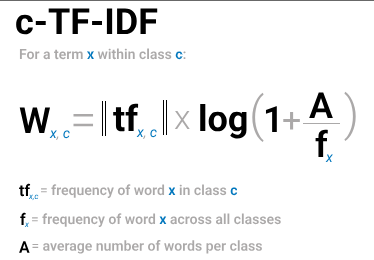
\includegraphics[width=0.4\textwidth]{images/tfidf.png}
    \caption{Modified version of TF IDF}
    \label{fig:tf-idf}
\end{figure}

This result would be importance scores for words within a cluster. The more important words are within a cluster, the more it is representative of that topic. In other words, if we extract the most important words per cluster, we get descriptions of topics.

Each cluster is converted to a single document instead of a set of documents. Then, we extract the frequency of word x in class c, where c refers to the cluster we created before. This results in our class-based tf representation. This representation is L1-normalized to account for the differences in topic sizes.

Then, we take the logarithm of one plus the average number of words per class A divided by the frequency of word x across all classes. We add plus one within the logarithm to force values to be positive. This results in our class-based idf representation. Like with the classic TF-IDF, we then multiply tf with idf to get the importance score per word in each class. In other words, the classical TF-IDF procedure is not used here but a modified version of the algorithm that allows for a much better representation.
\chapter{Imperical results}

\startcontents[chapters]
\printmyminitoc{
}

To do the evaluation, I created similarity matrices to see if topics between clusters were well-separated. The more light color the matrices, the more clusters are being well separated. The score is created by the tf-idf score and we calculate using the Euclidean distance.


\section{MiniLMv2 representation}

The results are very promising. The list of the words after this technique is the theme that right now agents label by hand. We also see that there are topics that are close to each other by the list of the tf-idf most significant words. For example:

\begin{itemize}
    \item euros, facture, mobile, payer, forfait, paye |  about invoices
    \item euros, facture, mois, factures, juillet, pour |  about invoices
    \item maroc, espagne, france, pars, algrie, utilise |  about roaming
    \item sim, code, carte, pin, bloqu, cartes, tlphone | problem with sim card
    \item internet, wifi, rseau, connexion, internet | problem with internet connection
\end{itemize}

However, we could also see that HDBSCAN and PCA are not well put together. The list of words in this case only contains really common words that could appear in any document.

\begin{figure}[H]
    \centering
    \begin{subfigure}{0.45\textwidth}
        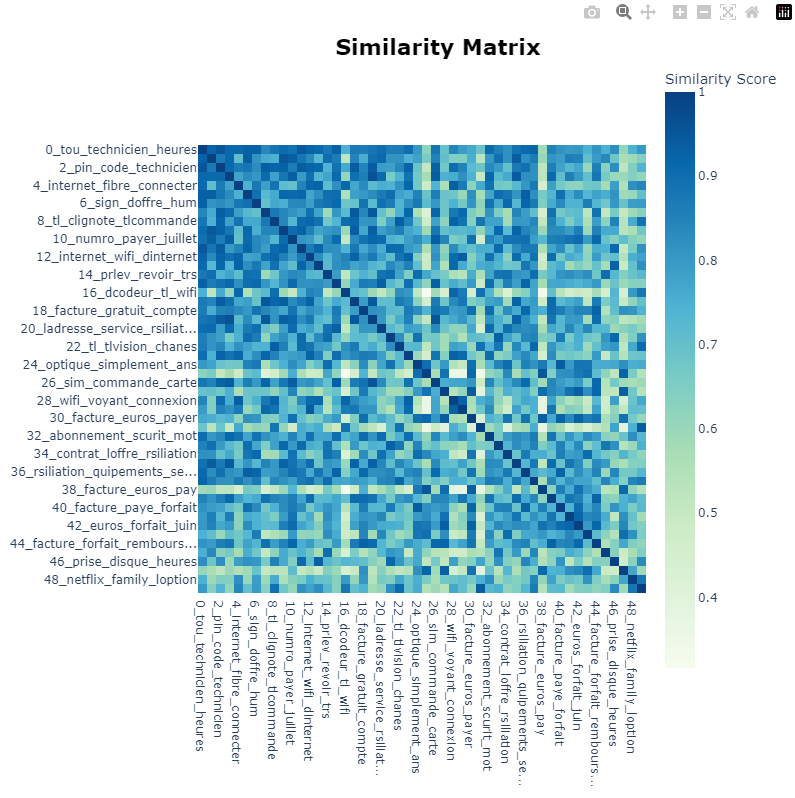
\includegraphics[width=\linewidth]{images/results/mini/kmeans_umap.png}
        \caption{Kmeans - UMAP}
    \end{subfigure}
    \begin{subfigure}{0.45\textwidth}
        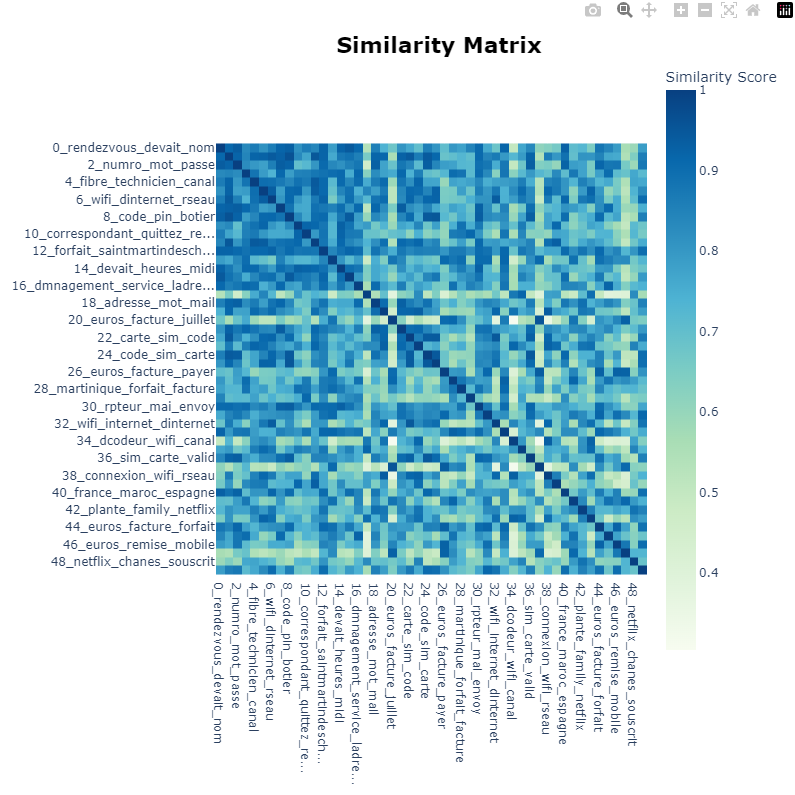
\includegraphics[width=\linewidth]{images/results/mini/kmeans_pca.png}
        \caption{Kmeans - PCA}
    \end{subfigure}
    \caption{Result - miniLMv2}
    \label{fig:result_mini_2}
\end{figure}


\begin{figure}[H]
    \centering
    \begin{subfigure}{0.45\textwidth}
        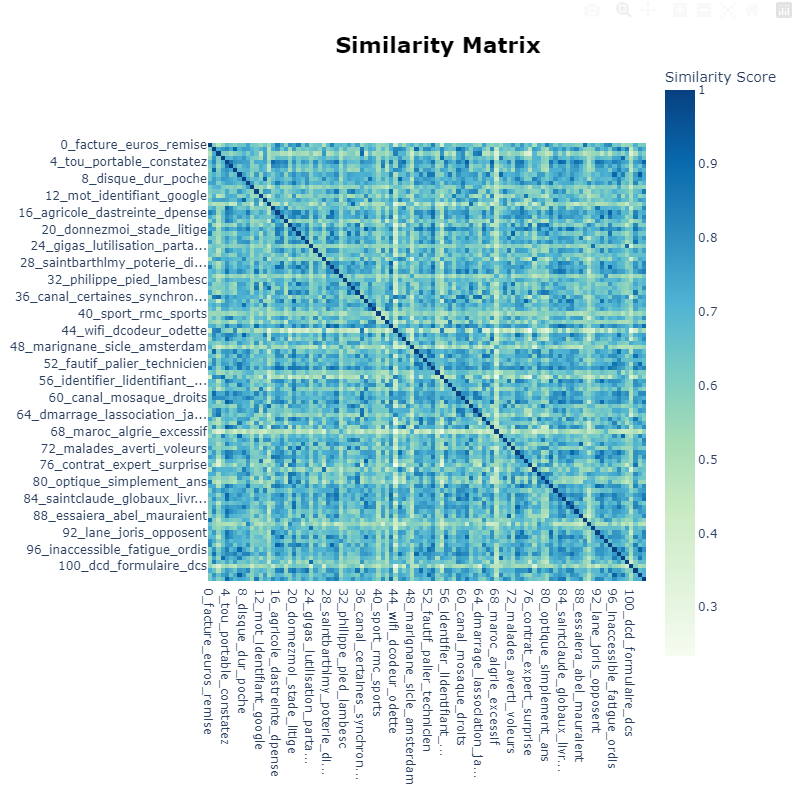
\includegraphics[width=\linewidth]{images/results/mini/hdbscan-umap.png}
        \caption{HDBSCAN - UMAP}
    \end{subfigure}
    \begin{subfigure}{0.45\textwidth}
        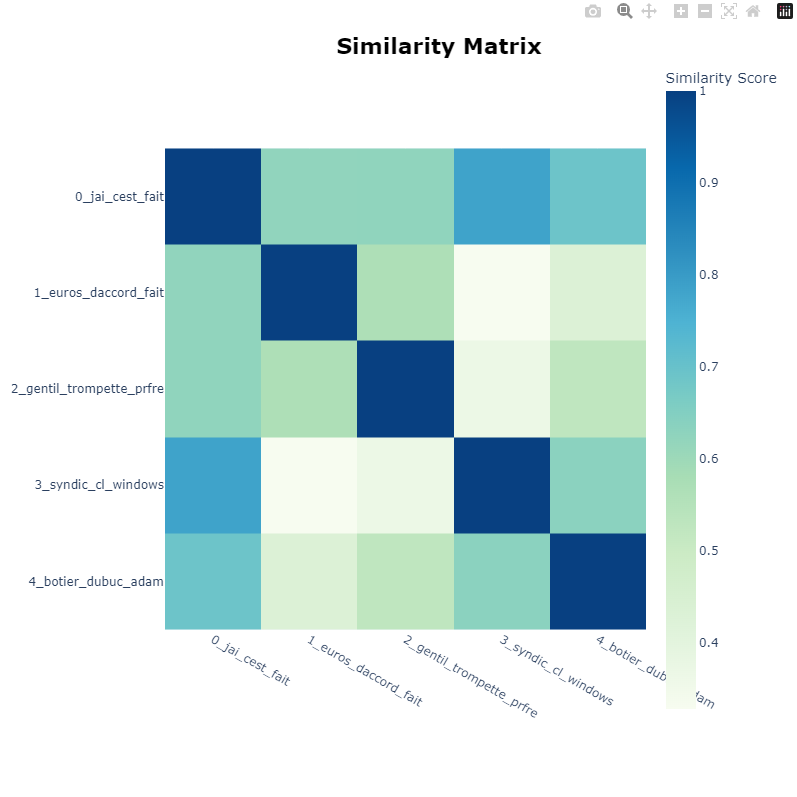
\includegraphics[width=\linewidth]{images/results/mini/hdbscan-pca.png}
        \caption{HDBSCAN - PCA}
    \end{subfigure}
    \begin{subfigure}{0.45\textwidth}
        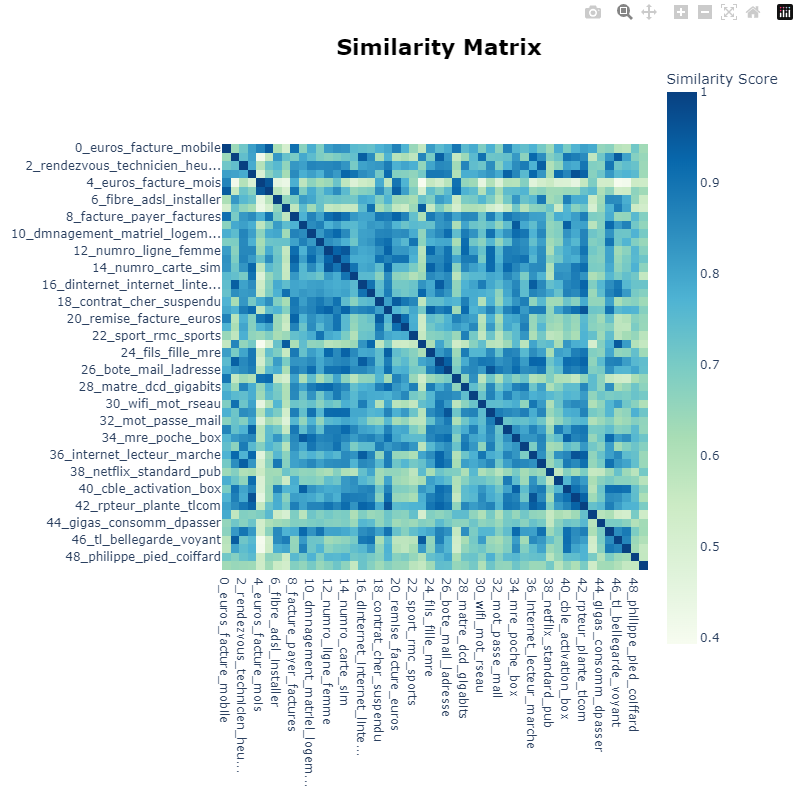
\includegraphics[width=\linewidth]{images/results/mini/hierachy_umap.png}
        \caption{Hierarchy - UMAP}
    \end{subfigure}
    \begin{subfigure}{0.45\textwidth}
        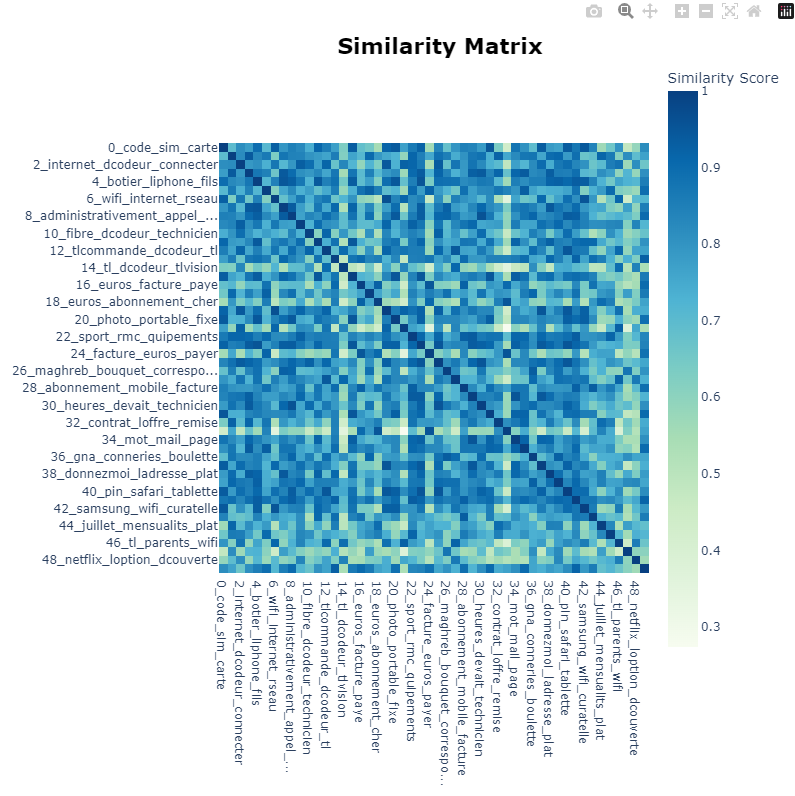
\includegraphics[width=\linewidth]{images/results/mini/hierachy_pca.png}
        \caption{Hierarchy - PCA}
    \end{subfigure}

    
    \caption{Result - miniLMv2}
    \label{fig:result_mini}
\end{figure}


\section{CamemBERT representation}

CamemBERT have a lower ability to distinguish between cluster than MiniLMv2. In the case of HDBSCAN and PCA with CamemBERT, because it is not obligated to cluster into mini clusters, it can even not separate clusters due to the close distance between data points.

% \begin{figure}[H]
%     \centering
%     \begin{subfigure}{0.43\textwidth}
%         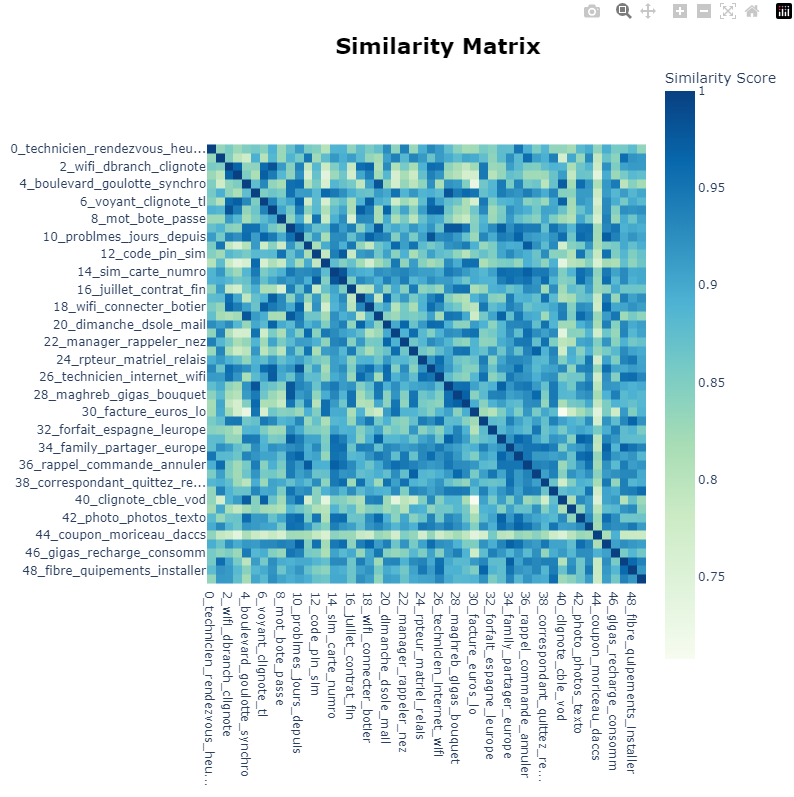
\includegraphics[width=\linewidth]{images/results/cam/kmeans_umap.png}
%         \caption{Kmeans - UMAP}
%     \end{subfigure}
%     \begin{subfigure}{0.43\textwidth}
%         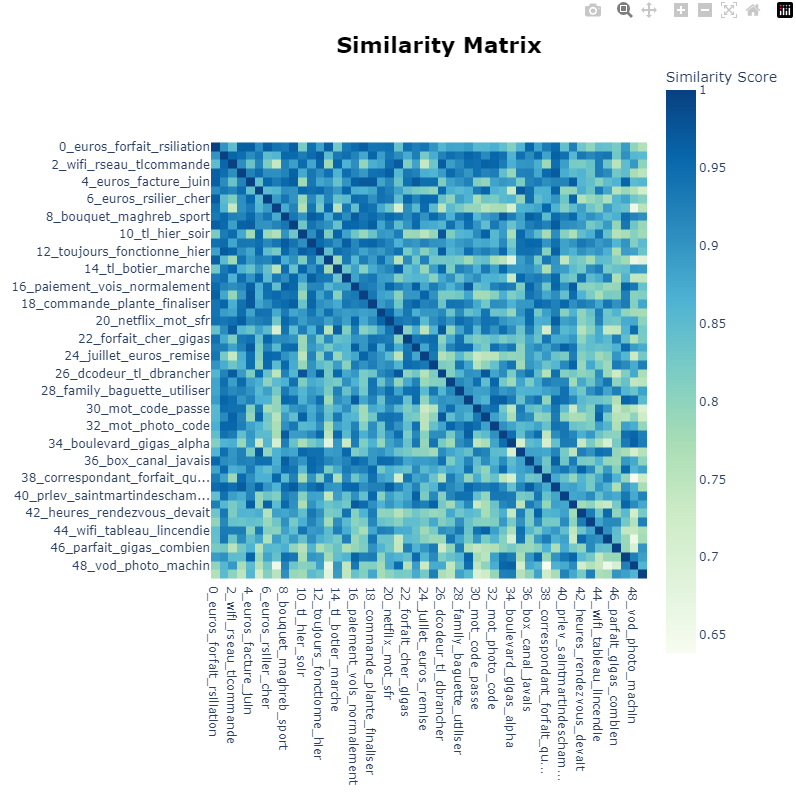
\includegraphics[width=\linewidth]{images/results/cam/kmeans_pca.png}
%         \caption{Kmeans - PCA}
%     \end{subfigure}
%     \caption{Result - CamemBERT}
%     \label{fig:result_cam_2}
% \end{figure}

\begin{figure}[H]
    \centering
        \begin{subfigure}{0.43\textwidth}
        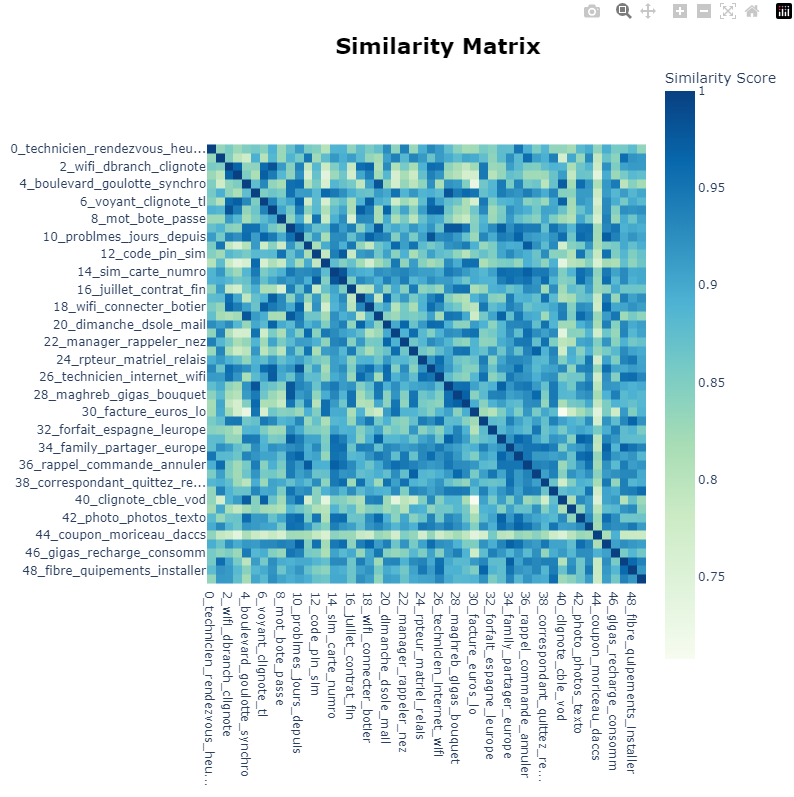
\includegraphics[width=\linewidth]{images/results/cam/kmeans_umap.png}
        \caption{Kmeans - UMAP}
    \end{subfigure}
    \begin{subfigure}{0.43\textwidth}
        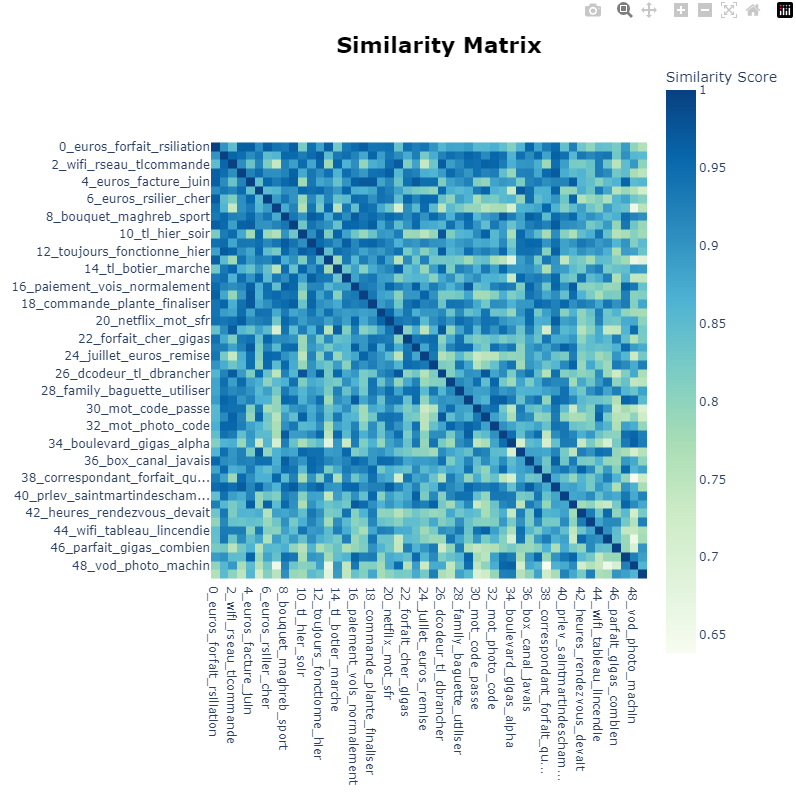
\includegraphics[width=\linewidth]{images/results/cam/kmeans_pca.png}
        \caption{Kmeans - PCA}
    \end{subfigure}
    \begin{subfigure}{0.43\textwidth}
        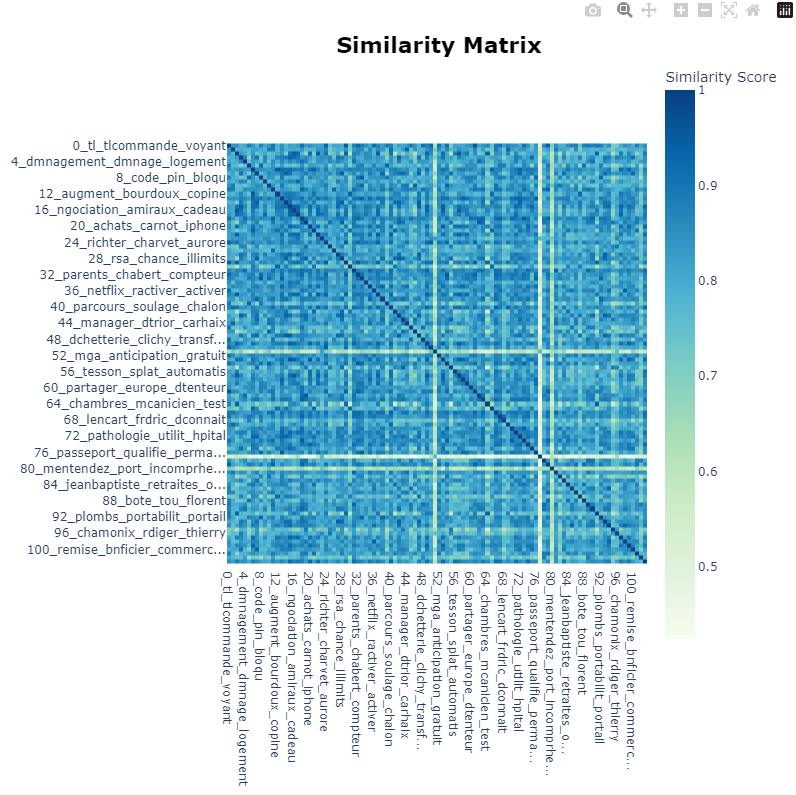
\includegraphics[width=\linewidth]{images/results/cam/hdbscan-umap.png}
        \caption{HDBSCAN - UMAP}
    \end{subfigure}
    \begin{subfigure}{0.43\textwidth}
        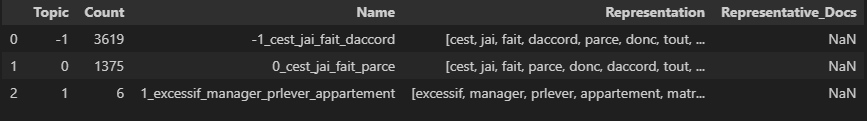
\includegraphics[width=\linewidth]{images/results/cam/hdbscan_pca.png}
        \caption{HDBSCAN - PCA}
    \end{subfigure}
    \begin{subfigure}{0.43\textwidth}
        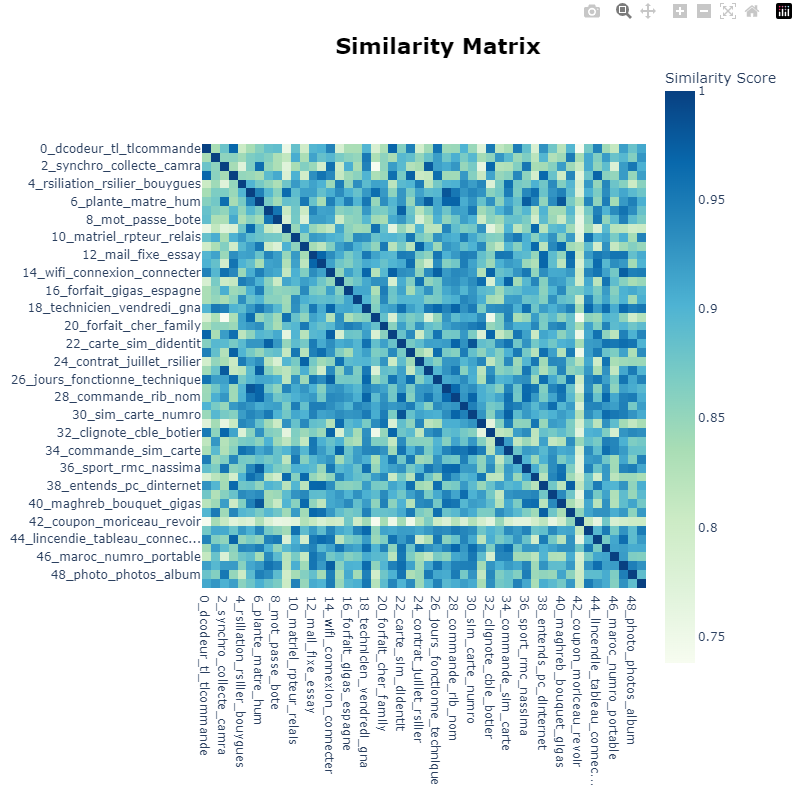
\includegraphics[width=\linewidth]{images/results/cam/hierachy_umap.png}
        \caption{Hierarchy - UMAP}
    \end{subfigure}
    \begin{subfigure}{0.43\textwidth}
        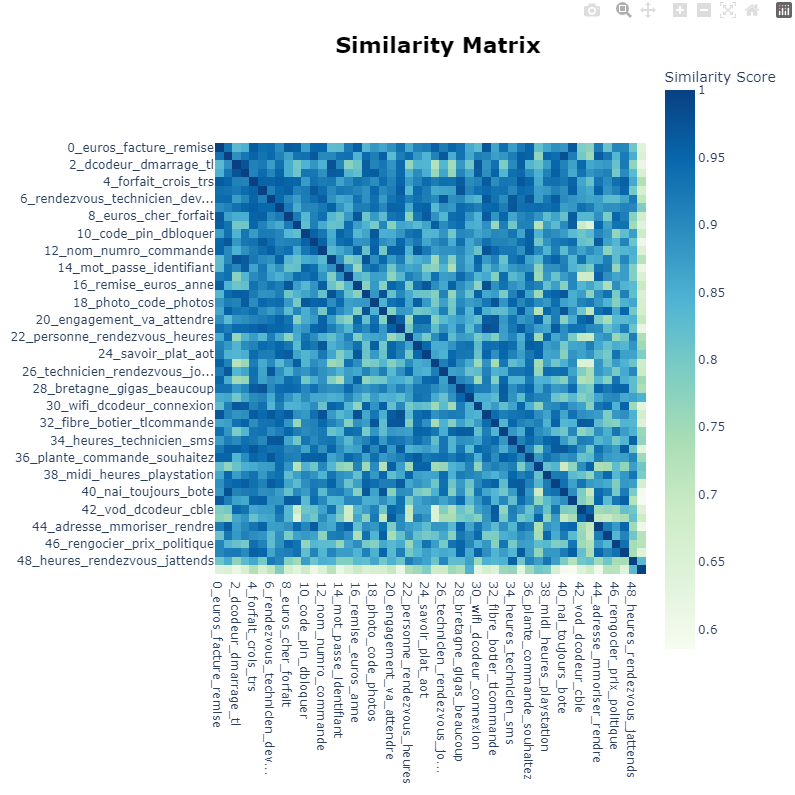
\includegraphics[width=\linewidth]{images/results/cam/hierachy_pca.png}
        \caption{Hierarchy - PCA}
    \end{subfigure}

    
    \caption{Result - CamemBERT}
    \label{fig:result_mini}
\end{figure}

\section{Hierarchy tree}

With this technique of representation, We can see which topics are closely related to each other. This is an example tree, using Hierarchy and UMAP

\begin{figure}[H]
    \centering
    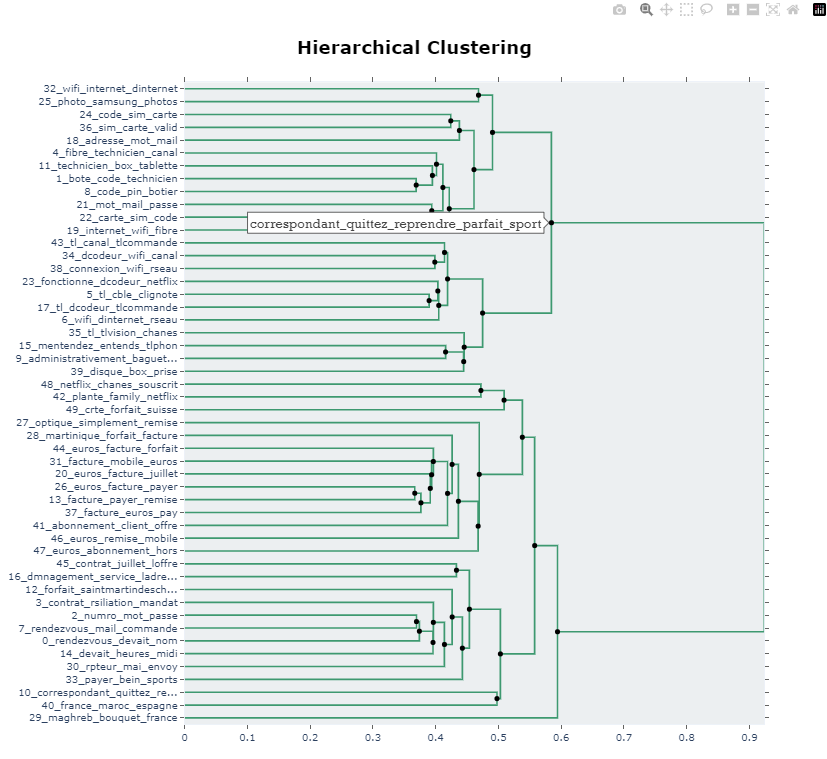
\includegraphics[width=1\textwidth]{images/results/mini/hierachy_umap_tree.png}
    \caption{Hierarchy - UMAP}
    \label{fig:hierachy_umap}
\end{figure}
\chapter{Conclusion and future works}

\startcontents[chapters]
\printmyminitoc{

}

\section{Conclusion}

We can see that in the tree of hierarchy clustering techniques, the most significant word of each topic is very promising. This method can cluster use cases in each small topic, with the cluster of technical problems, or the cluster of invoices, etc. being very well separated. 

There are many parameters in this method to adjust to find the best set out of it. After a dozen experiments, it is almost certain that MiniLMv2 performs better than CamemBERT. We can notice that in the similarity matrix between topics, the CamemBERT case is not very distinguishable between topics compared to MiniLM2. With the representation of the similarity matrix, we can also see that the technique that is the best in separating topics could be HDBSCAN. it is also not necessary for us to choose the number of clusters before but HDBSCAN can choose it.

This method still has some drawbacks. With one conversation, it could only be classified as one topic. However, in reality, One conversation could contain multiple topics at the same time. The customer could call the call center for multiple reasons or multiple problems. This point should be a point to focus on and research in the future of this project.

\section{Future works}

While our current topic modeling implementation has provided valuable insights, exploring hyperparameter tuning could significantly enhance the quality of topics extracted from the corpus. Investigating the optimal values for parameters such as the number of topics in Kmeans and hierarchy clustering, or different combination of UMAP and PCE could lead to more accurate and coherent topic assignments. Adopting techniques like cross-validation and grid search can systematically identify the hyperparameters that best capture the underlying structure of the data.

To extend the utility of our topic modeling system beyond our immediate team, the creation of an API (Application Programming Interface) could allow other teams and applications to integrate topic modeling functionality into their workflows. By providing an API, we enable seamless access to the topic modeling capabilities, enabling other teams to incorporate topic analysis within their projects without needing to delve into the technical intricacies of our model. The team in charge of building the interface for the agent could upgrade their product and call our API to suggest to the user the most significant word, making it easier for them when labeling the calls.


\pagebreak 
\appendix

\chapter{Example of original, soft clean, and hard clean text}
% \section{Appendix: }

\begin{itemize}
    \item \textbf{Original}
    
    oui monsieur bonjour j'ai un problème avec ma ligne fixe euh je le note oui oui oui oui oui c'est-à-dire que je je n'arrive pas à téléphoner que vous avez un numéro mais ça sera pas ça donne rien du tout sais plus comment j'ai pas compris monsieur je vais vous dire depuis au moins 3 ou 4 jours alors j'avais une personne chez vous qui m'a dit que y'avait un problème sur le réseau que ça allait être solutionné mais en fin de compte j'avais pas du tout oui à londres et je suis obligée de téléphoner de mon portable parce que ça fonctionne pas voilà andré redacted exactement oui oui oui absolument oui avec la télévision sachez euh la personne n'a été très très très patiente très aimable euh je suis arrivé à à ce que je voulais mais par contre je vais vous dire une chose euh avec la ligne et ma grande télévisions pour laquelle qu'on a j'ai eu un technicien qui est venu qui a changé la box euh j'arrive à l'allumer mais avec beaucoup de temps y'a y'a toujours un petit problème voilà d'accord le voyant du téléphone de du téléphone fixe le voyant euh sur ma banque j'ai dit 4 oui oui oui il est allumé est allumé non non mais je qui est pas je je l'ai fait deux fois je l'ai comme j'ai une personne la dernière fois qui m'a dit de débrancher rebrancher j'ai débranché j'ai rebranché quand je je je l'ai le téléphone je le remets ça fait un bruit mais je ne peux pas téléphoner ce téléphone je n'arrive pas à téléphoner je fais un numéro ça sonne pas rien le seul euh je pense que je sais pas comment attendez vous allez m'appeler sur le fixe ah ouais on les a d'accord essayez attendez attendez là le a pas accès c'est la box elle est éteinte allô elle est éteinte là y'a beaucoup de de de voyant qui j'arrive tout est éteint voilà la box est rallumé que vous voyez un téléphone oui la petite boîte blanche là y'a qu'une lumière habituellement y'en a 3 ma ma mais je d'accord ah d'accord très bien d'accord je suis à côté j'attends

    \item \textbf{Hard clean}
    
    j'ai problème ligne fixe note c'est-à-dire n'arrive téléphoner numéro ça ça donne rien tout sais plus comment j'ai compris vais dire depuis moins jours j'avais personne chez m'a dit y'avait problème réseau ça allait être solutionné fin compte j'avais tout londres obligée téléphoner portable parce ça fonctionne andré exactement absolument télévision sachez personne n'a très très très patiente très aimable arrivé voulais contre vais dire chose ligne grande télévisions laquelle qu'on j'ai technicien venu changé box j'arrive l'allumer beaucoup temps y'a y'a toujours petit problème d'accord voyant téléphone téléphone fixe voyant banque j'ai dit allumé allumé l'ai fait deux fois l'ai comme j'ai personne dernière fois m'a dit débrancher rebrancher j'ai débranché j'ai rebranché quand l'ai téléphone remets ça fait bruit peux téléphoner téléphone n'arrive téléphoner fais numéro ça sonne rien seul pense sais comment attendez allez m'appeler fixe ouais d'accord essayez attendez attendez là accès c'est box éteinte éteinte là y'a beaucoup voyant j'arrive tout éteint box rallumé voyez téléphone petite boîte blanche là y'a qu'une lumière habituellement y'en d'accord d'accord très bien d'accord côté j'attends

    \item \textbf{Soft clean}
    
    j'ai un problème avec ma ligne fixe je le note c'est-à-dire que je je n'arrive pas téléphoner que vous avez un numéro mais ça sera pas ça donne rien du tout sais plus comment j'ai pas compris je vais vous dire depuis au moins ou jours j'avais une personne chez vous qui m'a dit que y'avait un problème sur le réseau que ça allait être solutionné mais en fin de compte j'avais pas du tout londres et je suis obligée de téléphoner de mon portable parce que ça fonctionne pas andré exactement absolument avec la télévision sachez la personne n'a été très très très patiente très aimable je suis arrivé ce que je voulais mais par contre je vais vous dire une chose avec la ligne et ma grande télévisions pour laquelle qu'on j'ai eu un technicien qui est venu qui changé la box j'arrive l'allumer mais avec beaucoup de temps y'a y'a toujours un petit problème d'accord le voyant du téléphone de du téléphone fixe le voyant sur ma banque j'ai dit il est allumé est allumé mais je qui est pas je je l'ai fait deux fois je l'ai comme j'ai une personne la dernière fois qui m'a dit de débrancher rebrancher j'ai débranché j'ai rebranché quand je je je l'ai le téléphone je le remets ça fait un bruit mais je ne peux pas téléphoner ce téléphone je n'arrive pas téléphoner je fais un numéro ça sonne pas rien le seul je pense que je sais pas comment attendez vous allez m'appeler sur le fixe ouais on les d'accord essayez attendez attendez là le pas accès c'est la box elle est éteinte elle est éteinte là y'a beaucoup de de de voyant qui j'arrive tout est éteint la box est rallumé que vous voyez un téléphone la petite boîte blanche là y'a qu'une lumière habituellement y'en ma ma mais je d'accord d'accord très bien d'accord je suis côté j'attends
\end{itemize}

\printbibliography
\addcontentsline{toc}{chapter}{Bibliographie}



\end{document}
